\documentclass{tufte-book}
\usepackage{mystyle-tufte}



\begin{document}



\frontmatter

\newpage\thispagestyle{empty}
\graphicspath{{/Users/bblais/Documents/img/}}
\maketitlepagewithimage{cover_draft2}

\newpage\thispagestyle{empty} \openepigraph{%
Faith is taking the first step even when you don't see the whole staircase.}{Martin Luther King, Jr.}
\vfill
\openepigraph{%
Life's most important questions are, for the most part, nothing but probability problems.
}{Pierre-Simon Laplace%, {\itshape Design, Form, and Chaos}
} \vfill
\openepigraph{%
Faith consists in believing when it is beyond the power of reason to believe.}{Voltaire}
\vfill

\ifx\citep\undefined
   \let\citep\cite
   \let\citet\cite
\else
   \renewcommand\citep{\cite} \renewcommand\citet{\cite} \fi

\maketitle

\newpage

\begin{fullwidth}
~\vfill
\thispagestyle{empty}
\setlength{\parindent}{0pt}
\setlength{\parskip}{\baselineskip}
Copyright \copyright\ \the\year\ \thanklessauthor

\par\smallcaps{Published by \thanklesspublisher}

\par\smallcaps{typeset with tufte-latex}

\par     This book is licensed under the Creative Commons
    Attribution-ShareAlike license, version 3.0, 
    \url{http://creativecommons.org/licenses/by-sa/3.0/},
    except for those photographs and
    drawings of which I am not the author, as listed in the photo credits.
    If you agree to the license, it grants you certain privileges that
    you would not otherwise have, such as the right to copy the book,
    or download the digital version free of charge from
    \url{http://web.bryant.edu/~bblais}. At your option, you may also copy this book
    under the GNU Free Documentation License version 1.2, http://www.gnu.org/licenses/fdl.txt,
    with no invariant sections, no front-cover texts, and no back-cover texts.
\index{license}

\par\textit{First printing, \monthyear.  Last Compiled \today.}
\end{fullwidth}

\cleardoublepage
\textasciitilde{}\vfill

\begin{doublespace}
\noindent\fontsize{18}{22}\selectfont\itshape
\nohyphenation
Dedicated to...
\end{doublespace}

\thispagestyle{empty} \vfill
\vfill

\cleardoublepage

\tableofcontents

\mainmatter

\chapter{Introduction}\label{introduction}

\begin{quote}
\emph{Life's most important questions are, for the most part, nothing
but probability problems.} - Laplace
\end{quote}

\section{Why write a book like this?}\label{why-write-a-book-like-this}

This book is written to address the role that the mathematics of
probability can play when applied to topics in religion. Specifically,
we have found that there are two primary purposes of this approach:

\begin{enumerate}
\def\labelenumi{\arabic{enumi}.}
\itemsep1pt\parskip0pt\parsep0pt
\item
  Bring clarity to other similar treatments of these topics. The
  mathematics of probability have, unfortunately, been used to give the
  veneer of authority and objectivity to Christian apologetic arguments
  that are not well supported\citep{swinburne2003resurrection}. This is
  typically done by sneaking, possibly inadvertently, a bad assumption
  into an otherwise correct analysis. Understanding the structure of the
  mathematics can help in correcting this.
\item
  Bring concreteness and lucidity to more verbose and \emph{murky}
  approaches. When talking about terms like \emph{faith},
  \emph{miracles}, and \emph{evidence}, the mathematics forces the
  analysis to be both specific and complete, while at the same time
  having the benefit of reducing the number of symbols used in the
  description. Thus, there is an economy of words that is achieved.
  Pages of philosophical exposition can often be summarized by a few
  equations\citep{howard2013propositional}. This makes it much easier to
  explore special cases, and to see where analogies are successful and
  where they fail. This process gives the reader the ability to see
  connections between concepts, even when they seem opposed.
\end{enumerate}

\section{Who is this for?}\label{who-is-this-for}

Although we intend this book to be technical, we do not want to scare
away those who are less mathematical. In fact, we would consider it a
success if someone who is not particularly inclined in the mathematical
arts would be able to get a new appreciation for these topics upon
reading this book. Therefore, we will try to limit the technical aspects
to those that are only absolutely necessary, and will rely heavily on
specific examples at all times.

\section{Organization}\label{organization}

In this chapter we outline the basics of probability, applied to a few
simple cases. We then explore in subsequent chapters the details of
specific concepts, including \emph{faith}, \emph{miracles}, and
\emph{historical methods}. Typically, these explorations center around
responses to particular works, podcast discussions and debates.

\section{Introduction to Probability}\label{introduction-to-probability}

When we speak about probability, we speak about a percentage chance
(0\%-100\%) for something to happen, although we often write the
percentage as a decimal number, between 0 and 1. If the probability of
an event is 0 then it is the same as saying that you are certain that
the event will never happen. If the probability is 1 then \emph{you are
certain that it will happen}. Life is full of uncertainty, so we assign
a number somewhere between 0 and 1 to describe our state of knowledge of
the certainty of an event. The probability that you will get struck by
lightning sometime in your life is \(p=0.0002\), or 1 out of 5000.
Statistical inference is simply the inference in the presence of
uncertainty. We try to make the best decisions we can, given incomplete
information.

Pierre-Simon Laplace, who first formalized the mathematics of
probability, spoke of an agent with perfect knowledge. This agent,
Laplace claimed, would not need probability at all.

\begin{quote}
We may regard the present state of the universe as the effect of its
past and the cause of its future. An intellect which at a certain moment
would know all forces that set nature in motion, and all positions of
all items of which nature is composed, if this intellect were also vast
enough to submit these data to analysis, it would embrace in a single
formula the movements of the greatest bodies of the universe and those
of the tiniest atom; for such an intellect nothing would be uncertain
and the future just like the past would be present before its
eyes.\citep{laplace1825philosophical}
\end{quote}

E.T. Jaynes describes it in much the same way. He says that we label
something ``random'' due to our ignorance of the system not to any
intrinsic randomness. He called this labeling the mind-projection
fallacy\citep{Jaynes2003}, where you misattribute the unpredictable
behavior of a system as a product of the system itself. A rolled die is
following the laws of physics, deterministically, and detailed knowledge
of the die, the roll, and the surface should allow you to predict 100\%
of the time what it will do. We lack that knowledge, thus the behavior
becomes unpredictable. We often then attribute that unpredictable
behavior as a ``random die'', as if it were the die that contains the
randomness and not our own ignorance.

\subsection{The Basic Rules of
Probability}\label{the-basic-rules-of-probability}

For a complete description of these rules, and their application in
general statistical inference there are several books available, one of
which from the present author\citep{Blais:2014aa}. We will need to
establish a basic set of notation and mathematics in order to address
the concepts. This notation will in some cases make clear and condensed
(due the terseness of mathematics) much longer expositions of the same
concepts in English. In other cases it will provide a systematic
framework for exploring disparate problems, in order to see the
connection to all of rational thought. We begin by describing the rules
of probability, and some of their consequences.

\subsubsection{Rule 1 (Definition rule):}\label{rule-1-definition-rule}

\(P(A)\) is a number between 0 and 1, representing the strength of
belief in a statement, \(A\).

An example is
\[P(\mbox{you will get struck by lightning sometime in your life}) = 0.0002\]

Although this probability is estimated by the fraction of people being
struck by lightning, whenever we write probabilities we are referring to
a measure of the strength of one's belief in a proposition. Thus, this
probability means that you believe it to be extremely unlikely that you
will be struck by lightning in your life. This belief, as we will see,
is not just a guess but is something arrived at through proper rational
processes, or in other words, by adhering strictly to the rules of
probability.

In terms of economy of symbols\footnote{Because this is just a
  shorthand, we find it useful when the formalism gets too abstract to
  insert whatever statement for the shortcut you want. Thus, it helps
  your intuition to put in a specific example with each equation.}, we
will often define a single symbol to represent an entire sentence, or
collection of sentences. For example,

means that you believe it to be extremely unlikely that you will be
struck by lightning in your life.

\subsubsection{Rule 2 (Negation rule):}\label{rule-2-negation-rule}

\[P(A) + P({\rm\bf not}\, A) = 1\] In other words, either a statement is
true or its negation is true. means that you can be certain that either
you will be struck by lightning in your life or you won't. This seems
rather obvious, and you may be wondering why we even bring it up, but it
becomes a source of one of the most common logical fallacies - the
either-or fallacy.

Notice how this occurs. The following is correct logical inference:
means that, if you draw a playing card from a deck, you can be
\emph{certain} that it is either black or it is not-black. This is true
no matter what kind of deck of cards you are dealing with. The
following, however, is not correct logical inference: The key point here
is that ``not-black'' is not the same as ``red'', except in those cases
where you can be certain that there are only those two possibilities.
One has to be on the lookout for hidden possibilities - perhaps one has
a \emph{Five Crowns} deck which has green and yellow cards as well.
Failure of imagination can easily lead to accidental either-or logical
failures\footnote{An example seen later is an argument by a Christian
  examining the probability of theism (\(T\)) being true or atheism
  (\(A\)) being true. The argument hinges on \(P(T)+P(A)=1\), and trying
  to reduce \(P(A)\) to win the argument. However, the proposition
  ``theism is true'' masks as many alternatives as ``not-black'' in the
  example here. One could have the Christian God, the Greek pantheon,
  the Cthulhu mythological structure, etc\ldots{} and thus the argument
  does not perform what the Christian thinks it does.}.

\subsubsection{Rule 3 (Conjunction
rule):}\label{rule-3-conjunction-rule}

\[\P{$A$ and $B$} = P(B|A)P(A)\] which is the probability of two
statements both being true, A \textbf{and} B. We define a new symbol,
\(|\), which should be read as ``given.'' When there is information
given, we call this probability \emph{conditional} on that information.

means that the chance of you getting struck by lightning in your
lifetime \textbf{and} you like to play golf in the rain is related to
the probability of you liking to play golf in the rain (\(P(G)\)) and
the probability that you will get struck by lightning in your lifetime
given that you like to play golf in the rain (\(P(H|G)\)). There are a
few points to be made here, which become important in later examples.

\begin{enumerate}
\def\labelenumi{\arabic{enumi}.}
\itemsep1pt\parskip0pt\parsep0pt
\item
  Notice how concise the description is - the math can summarize the
  relationship between several concepts with few words or symbols.\\
\item
  \(P(H|G)\) is probably higher than \(P(H)\). In other words, the fact
  that a person likes to play golf in the rain makes it more likely that
  they will be struck by lightning in their lifetime.
\item
  Even if we don't have specific numbers, we can still reason about
  which probabilities are larger or smaller, or which ones are important
  or not.
\item
  \(P(H \mbox{ and } G)\) is \emph{always} less than \(P(G)\) - the
  conjunction of two things is inherently (and mathematically) less
  probable than the individual components\footnote{Sam Harris likes to
    humorously point out that Mormonism is \emph{objectively} less
    likely than Christianity because Mormonism is Christianity
    \textbf{and} a number of implausible statements. This, however, is
    somewhat misleading because Christianity is also predicated on those
    so-called implausible statements being false. One has to be careful
    when constructing the probabilities!}.
\end{enumerate}

\subsubsection{Rule 4 (Bayes' rule):}\label{rule-4-bayes-rule}

This rule is perhaps the most obtuse to see for the first time, but is
by far the most important rule of them all, so it is worth the effort.
Because of this, we will choose to write it in a somewhat more
elaborated form, and rewrite it several ways.

\begin{eqnarray*}
\Pg{explanation}{data} = \frac{\Pg{data}{explanation}\P{explanation}}{\P{data}}
\end{eqnarray*}

where each term is described more fully as

\begin{enumerate}
\def\labelenumi{\arabic{enumi}.}
\itemsep1pt\parskip0pt\parsep0pt
\item
  \(\P{explanation}\) - this is the probability the explanation is
  correct \emph{prior} to seeing the data. The term itself is often
  called the \emph{prior}, and represents your beliefs before you see
  the data. Typically, more complex explanations are less likely
  a-priori than simpler ones.\\
\item
  \(\Pg{explanation}{data}\) - this is the probability the explanation
  is correct \emph{after} seeing the data (a-posteriori). The term
  itself is often called the \emph{posterior} for this reason, and
  represents your updated beliefs once you have data. Thus, Bayes' rule
  is a mathematical expression of \emph{learning} from evidence.\\
\item
  \(\Pg{data}{explanation}\) - this is the probability that the data can
  be explained with this particular explanation. The term itself is
  often called the \emph{likelihood}, and can be thought of as a measure
  of how well the explanation fits the data. If the explanation fits the
  data well, this number will be high, for example.
\item
  \(\P{data}\) - this is the probability of the data, regardless of the
  explanation. It is easiest to understand this term with an example.
\end{enumerate}

Imagine we are playing a game with several small decks of
cards\footnote{The analogy here is that the universe is set up with a
  set of rules that we are trying to determine. Thus, deciding on which
  deck we are holding is analogous to deciding which universe we are in
  given my observations of the universe. In other words, providing an
  \emph{explanation} of the data is really about determining which of
  the many possible universes we are in.}, defined here:

\begin{enumerate}
\def\labelenumi{\arabic{enumi}.}
\itemsep1pt\parskip0pt\parsep0pt
\item
  \(E_1: A\spades, 2\hearts, 3\spades,4\spades\)
\item
  \(E_2: A\hearts, 2\hearts, 3\spades, 4\spades\)
\item
  \(E_3: A\hearts,2\hearts, 2\hearts,4\spades\)
\item
  \(E_4: A\hearts,3\spades, 3\spades, 4\spades\)
\end{enumerate}

In the game, someone has handed us one of the decks, but we don't know
at all which one it is. We then draw the top card, observe that it is a
\(3\spades\), and see if we can reason about which deck is likely to be
the one we are holding. We choose such a small, simple system because it
is easy to intuit the answers without the math. This intuition can
provide a scaffold for understanding the mathematics, which can be used
in more complex examples where one \emph{doesn't} have a strong
intuition. It is therefore worth going through at least one example in
detail.

To begin, we need to assign the probabilities of the four cases
\emph{prior} to the data. Given total ignorance, we assign equal
probabilities to the four cases

\begin{eqnarray*}
P(E_1)&=&1/4 \\
P(E_2)&=&1/4 \\
P(E_3)&=&1/4 \\
P(E_4)&=&1/4
\end{eqnarray*}

The following are our intuitions, with the mathematics in parallel
below. Since we drew a \(3\spades\), our intuition says that this should
rule out \(E_3\) altogether. Further, it says \(E_4\) should be more
likely than the other remaining two because it contains the observed
card, \(3\spades\), more than one time - it is easier to get that
particular card from the fourth deck than the others.

The mathematics would look like this

\begin{eqnarray*}
P(E_1|3\spades)&=&\frac{P(3\spades|E_1)P(E_1)}{P(3\spades)}\begin{array}{c}\ \\\leftarrow\mbox{this term the same in all}\end{array}\\
P(E_2|3\spades)&=&\frac{P(3\spades|E_2)P(E_2)}{P(3\spades)}\\
P(E_3|3\spades)&=&\frac{P(3\spades|E_3)P(E_3)}{P(3\spades)}\\
P(E_3|3\spades)&=&\frac{P(3\spades|E_4)P(E_4)}{P(3\spades)}
\end{eqnarray*}

where we already have

\begin{eqnarray*}
P(E_1)=P(E_2)=P(E_3)=P(E_4)=1/3
\end{eqnarray*}

Further, we have

\begin{eqnarray*}
P(3\spades|E_1) = 1/4
\end{eqnarray*}

because one card out of 4 in the first deck is the \(3\spades\).
Likewise, we have

\begin{eqnarray*}
P(3\spades|E_2) &=& 1/4\\
P(3\spades|E_3) &=& 0 \\
P(3\spades|E_4) &=& 2/4 
\end{eqnarray*}

Finally we have

\begin{eqnarray*}
P(3\spades) = 4/16
\end{eqnarray*}

because there are \(``3\spades''\) cards out of all the 16 in the game.
Plugging these numbers in to the above equations, and performing the
arithmetic, we have

\begin{eqnarray*}
P(E_1|3\spades)&=&\frac{(1/4)\times (1/4)}{(4/16)} = 1/4 \\
P(E_2|3\spades)&=&\frac{(1/4)\times (1/4)}{(4/16)} = 1/4 \\
P(E_3|3\spades)&=&\frac{(0)\times (1/4)}{(2/12)} = 0 \\
P(E_4|3\spades)&=&\frac{(2/4)\times (1/4)}{(4/16)} = 1/2 \\
\end{eqnarray*}

which perfectly matches our intuition. Notice further that
\(P(3\spades|E_1)\) is another way of saying ``how well is the
observation of a \(3\spades\) explained by the idea that we're holding
the first deck?'' The entire process can then be thought of as updating
our initial beliefs with the new evidence.

\begin{quote}
\emph{Any process of reasoning, in any field whatsoever, is either
consistent with this process of calculation or it is not rational.}
\end{quote}

It is for this reason that we explore this process in such detail.

On another front, an alternate way to have calculated the shared bottom
term, \(P(3\spades)\), is the following Why would one write it in this
seemingly long-winded and complex way? Because it makes it easier to
say, in words, what this term is doing. It is the sum of all of the
probabilities for how well each explanation accounts for the data scaled
by how likely that explanation was before seeing the data. In other
words, proper rational inference requires that you re-weight the
strength of your beliefs in an explanation not just by how well that
explanation describes your observations, but also by how intrinsically
likely that explanation is before your observations and how well all of
the \emph{alternatives} perform on those same observations. An
observation can be very well explained by a particular explanation, but
if it can be equivalently explained by other, simpler, explanations,
then your belief in that more complex explanation may in fact
\emph{weaken} with the new observation (i.e.~it's probability could go
down).

\section{Defining Terms}\label{defining-terms}

Clearly the terms simplicity, belief, knowledge, and proof are related
but it is the framework of probability that helps us be specific about
their differences. We can summarize the situation with the following,

\begin{itemize}
\itemsep1pt\parskip0pt\parsep0pt
\item
  \emph{Simplicity} refers to the flexibility of a model or hypothesis.
  The \emph{simpler} one is less flexible.
\item
  \emph{Belief} is measured by probability. Higher probability is
  equivalent to stronger belief, and likewise, lower probability is
  equivalent to weaker belief.
\item
  \emph{Knowledge} is a subset of belief, described more specifically
  below.
\item
  \emph{Proof} refers specifically to the result of a \emph{deductive}
  process. In this process, one starts with some (given) axioms, and can
  demonstrate \emph{with certainty} (i.e.~prove) a number of theorems
  (i.e direct consequences) from those axioms. Thus, the word proof
  should only be used in situations involving \emph{certainty}, or in
  other words, probabilities of exactly 1 or exactly 0 only.
\end{itemize}

The following explores these terms in more detail.

\subsection{Simplicity}\label{simplicity}

Ockham's razor, which is the philosophical idea that simpler theories
are preferred, is a consequence of Bayes' rule when comparing models of
differing complexity\citep{jefferys1991sharpening}. We can see this by
extending the card game example with a fifth possibility. Instead of
giving the specific cards in this deck, we are simply told

\begin{enumerate}
\def\labelenumi{\arabic{enumi}.}
\itemsep1pt\parskip0pt\parsep0pt
\item
  \(E_5:\) the deck can have anywhere from zero to three \(3\spades\),
  and enough other cards to make a total of four cards
\end{enumerate}

This explanation of the game is plastic - depending on the data, we may
infer a different value for the number of \(3\spades\) in this
deck\footnote{In mathematical models, this is often referred to as
  having an \emph{adjustable parameter} - a value in the model that is
  not specified ahead of time, but can be \emph{fit} to the data, and an
  optimum value found.}. It may be heavily loaded toward \(3\spades\),
which would make \(E_{5}\) explain the data very well; however it may
have none, and not explain the data at all. Clearly, once you observe a
\(3\spades\), the ``best'' value for this deck is to have three of them
out of the four cards - making it more likely than the previously best
explanation, \(E_4\), which only had two our of four.

However, this process of reasoning violates the laws of probability by
not taking our uncertainty of this parameter (i.e.~the number of
\(3\spades\) in the deck) into account. For simplicity, let's just
consider the two decks in question, \(E_4\) and \(E_5\), and play the
game with them (again, as before, drawing a \(3\spades\) from the top).

\begin{enumerate}
\def\labelenumi{\arabic{enumi}.}
\itemsep1pt\parskip0pt\parsep0pt
\item
  \(E_4: A\hearts,3\spades, 3\spades, 4\spades\)
\item
  \(E_5:\) the deck can have anywhere from zero to three \(3\spades\),
  and enough other cards to make a total of four cards
\end{enumerate}

We set up the calculation as before

\begin{eqnarray*}
P(E_4|3\spades)&=&\frac{P(3\spades|E_4)P(E_4)}{P(3\spades)}\\
P(E_5|3\spades)&=&\frac{P(3\spades|E_5)P(E_5)}{P(3\spades)}
\end{eqnarray*}

We defer the calculation of the shared term, \(P(3\spades)\), and focus
on the numerators of both
calculations.\marginnote{Once we have the numerators, we can add them up to get the shared term $P(3\spades)$}
First the one for \(E_4\) (and remember, we have only two decks here),

\begin{eqnarray*}
P(E_4|3\spades)&\sim&P(3\spades|E_4)P(E_4)\\
&=&(2/4)\times (1/2) = 1/4
\end{eqnarray*}

Next with the \(E_5\) deck,

\begin{eqnarray*}
P(E_5|3\spades)&\sim&P(3\spades|E_5)P(E_5)\\
&=&\underbrace{P(3\spades|E_5)}_{\parbox{1.4in}{broken up into the four possibilities from zero to three $3\spades$}}\times (1/2) \\
\end{eqnarray*}

Each of the possibilities (all equally likely, because we are given no
other information) has the form of the fraction of \(\spades\) for that
possibility times 1/4 because there are 4 total possibilities to
consider, for example

\begin{eqnarray*}
P(3\spades|E_5\mbox{ {\bf and zero }} 3\spades)P(\mbox{zero } 3\spades|E_5) &=& \underbrace{(0/4)}_{\mbox{\#}\spades} \times (1/4)
\end{eqnarray*}

Doing the same for all the possibilities, we get for the \(E_5\)
numerator,

\begin{eqnarray*}
P(3\spades|E_5)P(E_5) &=&\left[(0/4)\times (1/4) +  (1/4)\times (1/4) +  (2/4)\times (1/4) +  (3/4)\times (1/4)\right]\times (1/2) \\
&=&3/16
\end{eqnarray*}

Finally, we can get the shared term,

\begin{eqnarray*}
P(3\spades)= 1/4 + 3/16 = 7/16
\end{eqnarray*}

and the probabilities of each of the decks, given the observation of a
\(P(3\spades)\),

\begin{eqnarray*}
P(E_4|3\spades)&=&\frac{1/4}{7/16} = 4/7\\
P(E_5|3\spades)&=&\frac{3/16}{7/16} = 3/7
\end{eqnarray*}

This means that, although \(E_5\) contains the \emph{possibility} of a
better fit to the data, it is less \emph{probable} because it has a
flexible parameter that is unspecified \emph{before} the data.

When we prefer a ``simpler'' model with Ockham's razor, simpler means
fewer such adjustable parameters. It also means that the predictions are
both\emph{specific} and not \emph{overly plastic}. For example, a
hypothesis which is consistent with the observed data, and also be
consistent if the data were the opposite would be overly plastic. An
example of an infinitely plastic ``explanation'' is \emph{magic did it}.
Because it can ``explain'' anything, given that it is consistent with
any possible observation, it explains nothing.

\subsection{Belief}\label{belief}

\begin{quote}
We say we believe a proposition \(A\) when \(P(A)>0.5\). We say we
believe \emph{strongly} in a proposition \(A\) when \(P(A)>0.95\) or
some other, somewhat arbitrary, high number. The strength of a belief is
a \emph{scale} measured my the probability assigned to that proposition.
\end{quote}

Everything we have covered so far in this book relates to belief.

\subsection{Knowledge}\label{knowledge}

What is knowledge? Plato gave the following definition of knowledge:

\begin{quote}
Knowledge is justified true belief.\citep{fine2003plato}
\end{quote}

This is an unsatisfying definition because, it seems, in order to
justifiably label anything as \emph{knowledge} with this definition we'd
need to be able to independently determine that the proposition is true.
This presupposes that there is some ``outside'' knowledge, which we feel
comes too close to assuming a religious justification at the outset. We
believe there is likely to be a truth to be known, but that we can never
truly know what it is for certain - but this is not a problem. It is a
red herring to bring up 100\% certainty for knowledge, because it is
never achievable, and isn't what we practically call knowledge\footnote{In
  this way, knowledge is a subset of belief.}. We prefer a definition
inspired by Stephen J Gould:

\begin{quote}
In science, `fact' can only mean `confirmed to such a degree that it
would be perverse to withhold provisional assent.' I suppose that apples
might start to rise tomorrow, but the possibility does not merit equal
time in physics classrooms.\citep{gould1981evolution}
\end{quote}

Where it says ``fact'', read ``knowledge''. Where it says ``science''
read ``life''. The fact, or knowledge, that the Sun rises in the east
and sets in the west is not due to a formal \emph{proof} that this is
always true, or will continue indefinitely into the future. It is an
admission that the probability is so outrageously high, given the
evidence of every other sun rise and sun set observed, and the further
confirmation of models of the solar system, that it would be ``perverse
to withhold provisional assent''. We accept the claim as a practical
matter, despite not being 100\% certain, because of the overwhelming
probabilities. This we call knowledge. It is thus never a problem to
admit lack of certainty in knowledge, and it can be seen as an obvious
diversion if anyone tries to argue in a manner that suggests it's a
problem.

Mathematically, we might write\footnote{\(P(A)\approx 1\) means that the
  probability of \(A\) is \emph{approximately} equal to 1} it as
\(P(A)>0.9999 \approx 1\). Notice that we don't need 100\% certainty to
claim knowledge, and that it is possible for the ``knowledge'' to be
wrong (although, by definition, it is highly unlikely for this to be the
case).

We can ask the question, how did we come to this knowledge? The answer
is simply, by applying the rules of probability! According to Bayes'
rule, we update our probabilities given the evidence. This can lead us
to approach, but never equal, probability of 1. We can approach, but
never achieve, complete certainty of any claim. Rationality only insists
that we apply the rules of probability systematically.

\subsection{Proof}\label{proof}

\subsection{Proof}\label{proof-1}

Do \emph{proof} and \emph{evidence} mean the same thing? No, they don't.
To summarize, proof refers specifically to the result of a
\emph{deductive} process. In this process, one starts with some (given)
axioms, and can demonstrate \emph{with certainty} (i.e.~prove) a number
of theorems (i.e direct consequences) from those axioms. Thus, the word
proof should only be used in situations involving \emph{certainty}, or
in other words, probabilities of exactly 1 or exactly 0 only.

Evidence, however, factors into inference through an \emph{inductive}
process, not \emph{deductive}. Induction is just another name for the
application of the rules of probability, so we have been doing that from
the beginning of the book. Deduction is just another name for formal
logic, where the probabilities are restricted to values of 0 or 1 only.
As a result, we have the following maxim,

\begin{quote}
\emph{Proof} does not exist in science, only in math and philosophy.
\end{quote}

The only place you can have proof is where you have \emph{axioms}
(i.e.~unprovable assertions), and can then \emph{prove} a number of
consequences of those axioms. We can prove, for example, that the sum of
the angles of a triangle is 180 degrees, if we start with the Euclidean
axioms of geometry. Science doesn't have axioms, and thus there are no
proofs - there is only evidence. We sometimes hear the term ``proven
scientifically'', even from people who should know
better\textbackslash{}footnote\{An example of someone who should know
better is Richard Carrier in his
\href{http://www.youtube.com/watch?v=YLvWz9GQ3PQ}{``Is Philosophy
Stupid'' talk}, his
\href{http://www.amazon.com/Proving-History-Bayess-Theorem-Historical/dp/1616145595}{books}
and his
\href{http://infidels.org/library/modern/richard_carrier/theory.html}{articles}.

Another way of putting it is that probability theory contains deductive
logic as a special case. As it applies to science, it has the following
consequence

\begin{quote}
All of the evidence in the universe cannot bring the probability of a
scientific claim to certainty.
\end{quote}

To see this directly, imagine we have two (and only two) hypotheses for
the Earth - flat earth and round earth. We can write Bayes' rule for the
probability of each given the data. Note that this data includes things
like the experience of airplane flight, Magellan's trip, pictures from
space - all of which could be faked! The flat earth hypothesis is not
\emph{logically} impossible, it's just been overwhelmed by the evidence.

\begin{eqnarray*}
P({\rm round}|{\rm data}) &=& \frac{P({\rm data}|{\rm round})P({\rm round})}{P({\rm data}|{\rm flat})P({\rm flat})+P({\rm data}|{\rm round})P({\rm round})}\\\\
P({\rm flat}|{\rm data}) &=& \frac{P({\rm data}|{\rm flat})P({\rm flat})}{P({\rm data}|{\rm flat})P({\rm flat})+P({\rm data}|{\rm round})P({\rm round})} 
\end{eqnarray*}

Notice that, no matter how well the round earth hypothesis explains the
data, \[P({\rm data}|{\rm round})\approx 1\] and how unlikely you
believe it is that the Earth is flat even \emph{before} the data,
\[P({\rm flat})\ll 1\] as long as there is some \emph{possible} (even if
seriously contrived) way to explain the data with the flat earth
hypothesis, \[P({\rm data}|{\rm flat}) \neq 0\] it is
\emph{mathematically impossible} to make the round earth hypothesis
certain, \[P({\rm round}|{\rm data})< 1\]

On the right-hand side of Bayes' Rule, the closer the round-earth terms
and the flat-earth terms get to 1 and 0, respectively, the closer the
left-hand terms get to 1 and 0, but they never \emph{equal} 1 and 0.
This does not mean that we can't be \emph{confident} of claims, only
that we cannot have \emph{absolute certainty of anything} in science
(and therefore, in life in general). Anyone who doesn't understand that
does not understand science.

For it to be \emph{reasonable to believe in something}, it must rise to
a level of probability that you would label it as \emph{belief}. Does
this ever happen, or should this ever happen, with untrue things?
Certainly. Here are a few that come to mind.

\begin{enumerate}
\def\labelenumi{\arabic{enumi}.}
\itemsep1pt\parskip0pt\parsep0pt
\item
  the world is flat - as long as you are constrained to not live near
  the shore, or see a lunar eclipse
\item
  life is designed - before the advent of Darwin's theory of natural
  selection
\item
  the Sun, and the stars, all go around the Earth - until the advent of
  physics
\end{enumerate}

In each of these cases there is in fact strong evidence for the claims,
and against the counter claims, to make it reasonable to believe them
(at the time). It is no longer reasonable to believe these claims - the
process of reason forces one to adjust the probabilities of the
hypotheses given new evidence, and to discard those hypotheses that
become too improbable.

\section{Lessons from Probability}\label{lessons-from-probability}

The mathematics of probability theory is the gold standard for all
statistical inference. It structures all inference in a systematic
fashion. However, it can be used without doing any calculations, as a
guide to qualitative inference. Some of the lessons that are
consequences of probability theory are listed here, and will be noted
throughout this text in various examples.

\begin{itemize}
\itemsep1pt\parskip0pt\parsep0pt
\item
  Confidence in a claim should scale with the evidence for that claim -
  the more evidence the higher confidence.
\item
  Ockham's razor, which is the philosophical idea that simpler theories
  are preferred, is a consequence of Bayes' Rule when comparing models
  of differing complexity that explain the data equally.
\item
  A complex model must explain the data \emph{better} than a simple
  model to be preferred.
\item
  Simpler means fewer adjustable parameters.
\item
  Simpler also means that the predictions are both \emph{specific} and
  not \emph{overly plastic}. For example, a hypothesis that is
  consistent with the observed data, and can also be consistent if the
  data were the opposite, would be overly plastic.
\item
  Your inference is only as good as the hypotheses (i.e.~models) that
  you consider.
\item
  Extraordinary claims require extraordinary evidence.\citep{sagandemon}
\item
  It is better to explicitly display your assumptions rather than
  implicitly hold them.
\item
  It is a \emph{good thing} to update your beliefs when you receive new
  information.
\item
  Not all uncertainties are the same.
\end{itemize}

There is not a universal agreement for the translation of numerical
probability values to qualitative terms in English (i.e.~highly
unlikely, somewhat unlikely, etc\ldots{}). One rough guide is shown in
Table\textasciitilde{}\ref{table1}. I will be following this convention
throughout the book, but realize that the specific probability
distinctions are a bit arbitrary.

\begin{longtable}[c]{@{}cc@{}}
\toprule
Term & Probability\tabularnewline
\midrule
\endhead
virtually impossible & 1/1,000,000\tabularnewline
extremely unlikely & 0.01 (i.e.~1/100)\tabularnewline
very unlikely & 0.05 (i.e.~1/20)\tabularnewline
unlikely & 0.2 (i.e.~1/5)\tabularnewline
slightly unlikely & 0.4 (i.e.~2/5)\tabularnewline
even odds & 0.5 (i.e.~50-50)\tabularnewline
slightly likely & 0.6 (i.e.~3/5)\tabularnewline
likely & 0.8 (i.e.~4/5)\tabularnewline
very likely & 0.95 (i.e.~19/20)\tabularnewline
extremely likely & 0.99 (i.e.~99/100)\tabularnewline
virtually certain & 999,999/1,000,000\tabularnewline
\bottomrule
\end{longtable}

\chapter{Simple Appllications}\label{simple-appllications}

In this chapter we explore a number of simple applications of the
framework of probability on topics in religion.

\section{Atheism and Agnosticism}\label{atheism-and-agnosticism}

Fewer words are as loaded and lead to as much disagreement on
definitions as the terms \emph{atheism} and \emph{agnosticism} do. In
this work, we will define these words in a particular way, which we find
the most consistent amongst the many different competing usages.

\begin{itemize}
\itemsep1pt\parskip0pt\parsep0pt
\item
  Theism and atheism refer to \emph{belief}
\item
  To be a \emph{theist} simply means to believe in one, or more,
  personal gods. This is in contrast to a \emph{deist} who believes in
  an impersonal god - a god that, for example, created the universe and
  then stands back and doesn't interact at all with it. As a result of
  this lack of interaction, deist beliefs are untestable - there can't
  be any consequences to measure a non-interacting god. Because of this,
  deist beliefs are not addressed at all in this book. Typically, we
  will be addressing the Christian or other monotheist arguments, but
  occasionally bring in polytheist beliefs as they apply.
\item
  To be an \emph{atheist} simply means that one does not \emph{believe}
  in the existence of any gods. It is a statement of being unconvinced.
  It is not a statement of confidence that there is no God, just that
  the arguments for the existence of God is unconvincing.
\item
  Gnosticism and agnosticism refers to \emph{knowledge} (which is a
  subset of belief)
\item
  \emph{Agnostics}{[}\^{}Sometimes an agnostic atheist is called a
  weak-atheist, and a gnostic atheist a strong atheist, but we find
  these terms a bit too pejorative to use.{]} believe that they cannot
  \emph{know} whether there is a God or not, whole \emph{gnostics} claim
  that \emph{knowledge} can be had for (or against) the existence of
  God. Thus, one can be an agnostic theist or agnostic atheist. Also
  note, that \emph{knowledge} is being used as described earlier, not as
  absolute certainty, but extremely high confidence.
\end{itemize}

An analogy can help sort things out. Say we have two explanations of the
number of stars, one that says there is an \emph{even} number of stars
and another that says there is an \emph{odd} number of stars. Pretty
much we know that, at any given instant, one of these \emph{must} be
true. However, strong belief in either one is completely unwarranted -
there is simply no way to know. From a probabilistic framework, we
express this as

\begin{eqnarray*}
P({\rm odd}) &=&0.5 \\\\
P({\rm even})&=&0.5
\end{eqnarray*}

Anyone making the strong claim that, for example, \(P({\rm even})>0.95\)
would have to present compelling evidence.

\begin{itemize}
\itemsep1pt\parskip0pt\parsep0pt
\item
  Someone who is an \emph{evenist} (analogous to a \emph{theist}) would
  be someone convinced by the evidence, and assigns a high probability
  for \(P({\rm even})\).\\
\item
  Someone who is unconvinced by the evidence, say, an \emph{a-evenist}
  (analogous to an \emph{a-theist}) could maintain a lower probability
  for \(P({\rm even})\).\\
\item
  A \emph{gnostic evenist} would have a very high probability for
  \(P({\rm even})\), while an \emph{agnostic evenist} would have a high,
  but not very high, probability for \(P({\rm even})\).\\
\item
  Likewise, a \emph{gnostic a-evenist} would have a very low probability
  for \(P({\rm even})\) (and thus a high \(P({\rm odd})\)), whereas an
  \emph{agnostic a-evenist} would have a low \(P({\rm even})\), and
  possibly equal to \(P({\rm odd})\).
\end{itemize}

Thus, for someone to be unconvinced of a ``claim'' (i.e. ``there are an
even number of stars'') because they find the evidence unconvincing
\emph{does not} entail that they have a \emph{belief} in the opposite
(i.e.~they do not necessarily believe there are an odd number of stars).
This point can't be made enough, because it is an extremely common
misunderstanding, typically by Christians about atheists.

Matt Dillahunty clearly defines atheism as a lack of belief, and in a
court-room analogy says that he finds God ``not guilty of existing''. In
court, you find the plaintiff ``guilty'' or ``not guilty'', not
``guilty'' or ``innocent''. The burden of proof lies squarely with the
prosecution. If they haven't met that burden, then the jury finds the
plaintiff ``not guilty''. They may, or may not, believe that the
plaintiff is innocent. Establishing \emph{innocence} in the crime
changes the burden of proof to the defendant. The difference here comes
down to priors, which we can see through some illustrative examples
mapped to probability.

\subsection{Different Data}\label{different-data}

If we imagine data that might actually affect this prior probability,
the situation is a bit different. Let's imagine that through the laws of
physics we could demonstrate that

\begin{enumerate}
\def\labelenumi{\arabic{enumi}.}
\itemsep1pt\parskip0pt\parsep0pt
\item
  stars are nearly always formed in pairs
\item
  single stars are very short-lived
\end{enumerate}

we may actually have an argument for an even-number of stars in the
universe. In this case, we have \[
P(O|{\rm data}) \ll P(O)
\] and thus \[
P(E|{\rm data}) \gg P(E)
\]

Where one belief goes down, the other goes up. For our belief in
odd-ness to go down our belief in evenness must go up. We no longer
simply \emph{lack} a belief in odd-ness we also both \emph{believe} in
even-ness and \emph{believe} in non-odd-ness.

\subsection{More than two outcomes}\label{more-than-two-outcomes}

Something interesting happens when there are more than two outcomes.

\[
P(H)=P(R)=P(Y)=\frac{1}{3}
\]

Some data that nearly rules out one hypothesis, say \(R\), may not speak
to either other hypothesis directly, so you get the equal redistribution
like:

\begin{eqnarray}
\nonumber P(R)&\sim& 0 \\\\ 
\nonumber P(H)=P(Y)&\sim& 1/2 
\end{eqnarray}

or it might be the case that the data leaves unchanged the prior
probability of one of the hypotheses, raising the probability of the
other, like

\begin{eqnarray}
\nonumber P(R)&\sim& 0 \\\\ 
\nonumber P(H)&\sim& 1/3 \\\\
\nonumber P(Y)&\sim& 2/3 
\end{eqnarray}

Notice that it is possible to reduce the probability of one hypothesis
(i.e. \(R\)) and not effect the probability of a separate hypothesis
(i.e. \(H\)), when there are more than two outcomes. It is also possible
for the probability of that separate hypothesis (i.e. \(H\)) to go up,
or even go down. In other words, when there are more than one
hypothesis, presenting evidence for (or against) one hypothesis does not
always guarantee an adjustment in another hypothesis down (or up).

\section{Avoiding the Veneer of
Objectivity}\label{avoiding-the-veneer-of-objectivity}

There is a danger of using mathematics to give the veneer of objectivity
to an argument that is riddled with random guesses, ill-defined
concepts, and unsupported premises. In this section, we analyze some
statements made in a podcast debate between theist Calum Miller and
atheist James Crofta, expressed as probability
statements\citep{Brierley:2014ab}.

\subsection{The Argument}\label{the-argument}

\ppquote{I think one useful way of thinking about is to consider
what evidence is in general. When we think about evidence for a theory,
in this case the theory is that God exists - we want to explain some
features of the world, we look for things (observations) which are
surprising if the theory isn't true but which aren't that surprising if
the theory is true.}{Calum Miller}

Calum Miller then goes on to do an analogy with fingerprints on a
murder\TODO{include?} weapon, as features of the world. He then points
out the observation what he believes is evidence for God.

\ppquote{There are a number of arguments that work this way. But one of
the particular pieces of evidence that we want to discuss today is that
the world exhibits a real kind of regularity and there are basic laws,
science works, that we can understand the world. For all we know, the
universe could have been chaotic, might not have been any laws at all,
we might not have been able to do science - it might have been complete
chaos.}{Calum Miller} \TODO{explain his quotes}

Here he's describing the form of the argument, as it might apply to the
sun rising.

\ppquote{Even more basic things that we use scientific reasoning for,
but do not always strike us as scientific truth. For example, *`the
sun will rise tomorrow'*. Most of us believe that; this is a
common-sense inference from our observations. On atheism there is no reason to expect that regularity, because the sun could just fail to rise tomorrow.  On theism we can expect that kind of regularity because God set it in place}{Calum Miller}

Calum Miller finishes by describing further how moral responsibility
hinges on this regularity, because we need to know the likely effect of
my actions on others in order to make moral decisions and be responsible
for them. If things were chaotic, if my actions had random effects, then
moral responsibility could not work.

\subsection{The problem with the math - posteriors vs
likelihoods}\label{the-problem-with-the-math---posteriors-vs-likelihoods}

The first problem with Miller's argument, from a math point of view, is
that he is simply comparing \emph{part} of Bayes' rule (i.e the
likelihoods, or how well the explanation fits the data) without looking
at the rest of Bayes' rule (i.e.~how likely, a-priori, those
explanations are). He compares the terms

\begin{eqnarray*}
\frac{P({\rm data}|{\rm theism})}{P({\rm data}|{\rm atheism})}
\end{eqnarray*}

and says that this is greater than one, and thus theism is more likely.
That is just the wrong question to ask. What we really want to look at,
even keeping the same structure, is the ratio of the \emph{posterior}
probabilities, or

\begin{eqnarray*}
\frac{P({\rm theism}|{\rm data})}{P({\rm atheism}|{\rm data})}
\end{eqnarray*}

which is related to the likelihood ratio through Bayes' rule:

\begin{eqnarray*}
\frac{P({\rm theism}|{\rm data})}{P({\rm atheism}|{\rm data})} &=& \frac{P({\rm data}|{\rm theism})}{P({\rm data}|{\rm atheism})} \times \frac{P({\rm theism})}{P({\rm atheism})}
\end{eqnarray*}

where we factor in the \emph{prior} probabilities. Already, we have an
issue, because the prior probability for the universe with an extra
agent should be smaller than one without such an
agent\footnote{Recall this as a consequence of the Conjunction rule above.}.
If you factor in the agent with many specific properties, then this is
smaller still. By omitting this part, you could argue for anything. For
example,

\begin{eqnarray*}
\frac{P({\rm data}|{\rm fairies})}{P({\rm data}|{\rm no-fairies})}>1
\end{eqnarray*}

or, in other words, the regularity of the universe is much more likely
given fairies than no-fairies, so that is evidence for the fairies. Even
if true, it is clearly an uninteresting and not a useful claim.

\subsection{The problem with the premise regarding
theism}\label{the-problem-with-the-premise-regarding-theism}

The next problem is that it seems that Calum Miller is trying to sneak
in many more details into his theism than his argument would warrant. He
needs to \emph{define} what he means by theism to state that it is more
likely to result in a regular universe. This is where the mathematics
forces one to be specific and thorough, and thus highlights problems in
arguments that may seem fine at their face.

For example, a number of counter examples can be made:

\begin{itemize}
\item  Under the Greek pantheon, it is more likely that things *would be chaotic*, at the will of capricious deities - thus $P({\rm data}|{\rm theism})$ would be lower than Calum Miller claims
\item  Gods or divine beings, such as Cthulhu, revel in chaos and thus would make it even less likely to result in a regular universe
\end{itemize}

So when Calum Miller says ``theism'', what he seems to mean is the
existence of ``order-making God(s)'', but then his argument is circular:
a regular universe is more likely under a regular-universe-making God
hypothesis than not.

\subsection{The problem with the premise regarding
atheism}\label{the-problem-with-the-premise-regarding-atheism}

Further, Calum Miller never supports that it is unlikely to have an
ordered universe under atheism. ``For all we know, the universe could be
chaotic'', Calum says. However, that needs to be \emph{demonstrated},
not asserted, or it is an argument from ignorance in disguise. It is
possible, and in fact cosmology seems to be pointing more in this
direction, that the universe could not be any other way - that the
regularity is the result of the production of any universe, and further
that the production of universes is the only stable solution. The notion
of philosophical ``nothing'' may not be physically realizable - it may
be impossible for ``nothing'' to exist.{[}\^{}Yes, I realize the verbal
tangles one gets into with using the word ``nothing'' in the same
sentence as ``exists''. Unfortunately, I doubt English can do much
better here.{]}

Calum Miller's introduction of morality to the argument adds nothing,
and only serves as a red herring. Without some regularity in the
universe, even thought itself would be impossible . We couldn't even
have the idea of a ``being'', or an animal, or life without regularity.
Thus, our mere existence requires regularity - but one that need not be
imposed from the outside, with a God.

So, in summary, introducing the notion of a generic theism causes more
problems to the argument than it solves, because it includes Zeus and
Cthulhu. Circularity results when restricting the relevant theism to
exclude these possibilities. Even if Calum Miller solved this, he is
still answering the wrong question by ignoring the prior probabilities,
and is at best achieving an uninteresting and useless result.

\section{Will the Sun rise tomorrow?}\label{will-the-sun-rise-tomorrow}

Continuing with the Miller-Croft debate, Miller eventually brings up the
analogy with evidence for the sun coming up as an example of knowledge
claims and models. The analogy fails when we look at the details of how
this evidence is calculated.

Calum Miller describes philosopher David Hume on the justification for
the sun rising tomorrow, and then continues with the analogy of model
building in this situation,

\pquote{Hume basically noted that we don't have any non-circular
justification for thinking that the universe will be regular, that it
will continue to be regular in the future.$\ldots$ He doesn't
just say that we have to be a bit unsure that the sun will rise
tomorrow, he says that we have no good reason at all for thinking the
sun will rise tomorrow. The most common justification that the sun will
rise tomorrow is that it has risen every day in the past. But then if
you compare two theories, one says that the sun rises everyday in the
past and in the future and the other theory says that the sun rises
everyday in the past but won't rise tomorrow. Both those theories
predict the observations we already have, both those theories lead us to
expect the observations, and so the observations we currently have don't
distinguish between these two theories. And yet one of those theories
predicts the sun will rise tomorrow and one of them predicts that the
sun won't rise tomorrow. So, even though we have those observations,
they don't really do an obviously good job of determining which of these
theories is true. $\ldots$ He is saying that the past observations
don't give us that good reason for thinking that the sun will rise
tomorrow. This is the Problem of Induction and has perplexed
philosophers for centuries.}

\subsection{What does Hume say?}

It is instructive to note that Hume predates the mathematics of
probability, and see what Hume \emph{actually} says about the Sun
rising\citep{Hume:1748aa}, \pquote{
Matters of fact, which are the second objects of human reason, are not
ascertained in the same manner; nor is our evidence of their truth,
however great, of a like nature with the foregoing. The contrary of
every matter of fact is still possible, because it can never imply a
contradiction, and is conceived by the mind with the same facility and
distinctness, as if ever so conformable to reality. That the sun will
not rise tomorrow is no less intelligible a proposition, and implies no
more contradiction, than the affirmation, that it will rise. We should
in vain, therefore, attempt to demonstrate its falsehood. Were it
demonstratively false, it would imply a contradiction, and could never
be distinctly conceived by the mind.}

Here Hume is essentially stating that all propositions have a non-zero
probability (however small they might be) unless they are
\emph{logically} impossible. This is not saying, at all, that we have no
good reason to believe the sun will rise tomorrow.

\pquote{The bread, which I formerly ate, nourished me: that is, a body of such
sensible qualities was, at that time, endued with such secret powers;
but does it follow, that other bread must also nourish me at another
time, and that like sensible qualities must always be attended with like
secret powers? The consequence seems nowise necessary.[@Hume:1748aa]
}

Again, although Hume predates probability theory, this is essentially
what he is saying - the consequence is not logically \emph{necessary}
(i.e. \(P({\rm consequence}|{\rm observations})<1\)). We see this as a
direct application of probability theory, a totally uncontroversial
application at that.

The so-called ``problem of induction'' to which Calum Miller refers is
not really a problem. It is a direct consequence of the mathematics of
probability, and thus is the result of mathematical axioms. Hume is not
claiming that there is \emph{no} good reason to see the consequence
following from the the observations, only that he is unable to find a
good reason,

\pquote{
The connection between these propositions is not intuitive. There is
required a medium, which may enable the mind to draw such an inference,
if indeed it be drawn by reasoning and argument. What that medium is, I
must confess, passes my comprehension, and it is incumbent on those to
produce it, who assert that it really exists, and is the origin of all
our conclusions concerning matter of fact.
}

The medium Hume refers to is simply the mathematics of probability,
something which post-dates Hume's writings. Hume was being honest that
he didn't see a way, and he did not claim that there was \emph{no
possible} way - that would be an ``argument from ignorance'' fallacy.

\subsection{What does Laplace say?}

Once we have probability theory, then we can actually do some simple
calculations concerning the probability of the sun rising tomorrow. Of
course these calculations are not a complete description of the problem,
but give the flavor of it. Laplace used the sunrise problem as an
example application of his Rule of Succession, which itself is derived
from the rules of probability. The calculation goes something like this.

\begin{itemize}
\itemsep1pt\parskip0pt\parsep0pt
\item
  Our model is that the sun rises with unknown probability $p$
\item
  Given complete ignorance of $p$ we assume an initial uniform
  probability (all values are equivalent)
\item
  The sun has risen every day for the written record, say, 10000 years
\item
  the probability for rising tomorrow, which is also the mean value of
  $p$ over the posterior probability, is given by the Rule of
  Succession[@Wikipedia:2015ab] (also known as the "assume one success and one
  failure"[@Blais:2014aa]):
\end{itemize}

\newcommand{\yr}{\mbox{year}}
\renewcommand{\day}{\mbox{day}}

\begin{eqnarray*}
P\left(\parbox{.7in}{rise\\tomorrow}\middle|\parbox{1in}{rose today,\\rose yesterday, \\$\ldots$,\\ on day 0}\right)&=&
\frac{10000 \yr \times 365 \day/\yr+1}{10000 \yr \times 365 \day/\yr+2}\\
&=&0.9999997
\end{eqnarray*}

It gets messier when you can't even assume that both a failure and a
success are possible, but it can still be done without any change to the
qualitative result.

Clearly we have quite good reasons to believe the that sun will rise
tomorrow.

\subsection{Two theories}\label{two-theories}

We go back to Calum Miller's two theories:

\pquote{
If you compare two theories, one says that the sun rises everyday in the
past and in the future and the other theory says that the sun rises
everyday in the past but won't rise tomorrow. Both those theories
predict the observations we already have, both those theories lead us to
expect the observations, and so the observations we currently have don't
distinguish between these two theories.
}

The situation for arguing a high probability of tomorrow's sun rise is
far more compelling, however, because our information is not simply that
the sun has risen in the past, but includes observations of the patterns
of the seasons, the predictions of the phases of the moon and Venus, and
a whole host of other factors which significantly increase the chance
the sun will rise. Laplace knew this well, and was using this example
not as a serious calculation, but as a pedagogical example.

As a consequence, both of Calum Miller's so-called theories do
\emph{not} predict the observations we already have - only one of them
does. Even if we accept just the observations for which both theories
are consistent in the past, one has to view this two-theory perspective
from the point of prediction. Imagine it's now tomorrow, and ``Theory
B'' doesn't work - so we modify it to say the sun won't rise
\emph{tomorrow} (the new tomorrow). That next day comes with a sunrise,
and this ``Theory B 2.0'' is wrong (again) and has to be modified
(again). It is clear that ``Theory B'' fails, and we should be less
confident in it. That's why, in science, it isn't nearly enough to be
consistent with past data - one must make predictions, not just
post-dictions, and test it. It is often trivial to come up with
``explanations'' for data we already have - especially when we can be
infinitely plastic in the models we propose.

\section{Belief, Knowledge, and Scientific
Literacy}\label{belief-knowledge-and-scientific-literacy}

Concepts about belief and knowledge arose in the National Science
Foundation survey on scientific literacy. The NSF had decided to change
the wording of two questions in the survey. The original wording is
\pquote{Human beings, as we know them today,
developed from earlier species of animals,} and
\pquote{The universe began
with a huge explosion.}

The new wording is \pquote{\underline{According to
evolutionary theory,} human beings, as we know them today, developed
from earlier species of animals"  (emphasis mine)} and
\pquote{\underline{According to astronomers,}
the universe began with a huge explosion." (emphasis mine)}

It is noted that there will be a transition period with the questions,
with half of the surveys containing the new questions and half the old,
to determine its effect.

The stated goal for this change, from the NSF, is to separate knowledge
from belief. You might \emph{believe} that humans are created in their
present form, 6000 years ago, but the new questions try to ascertain
whether you know that ``evolutionary theory'' says something different.
Is this an important distinction? Is this what we really want to
measure? Which is more important for a society? What is the difference
between knowledge and belief in this context?{[}\^{}It is quite clear
that there will be at least one effect for this rewording: given that
the US falls way behind other countries on science literacy, especially
with these particular questions, the rewording will most likely increase
these numbers with no other work done.{]}

Since beliefs are representations of the world that we hold to be
correct for the real world\ldots\{\}as opposed to hopes, which are also
representations of the world but not ones that we hold to be necessarily
correct. Knowledge is, as we have defined, simply that collection of
beliefs that we hold with such high probability or, in other words, with
such confidence that we do not significantly doubt them. The belief that
the sun rises in the east each morning is considered knowledge for the
reason that we hold it with an extremely high probability.

The NSF defines scientific literacy as
\href{http://www.nsf.gov/statistics/seind04/c7/c7s2.htm}{"knowing basic
facts and concepts about science and having an understanding of how
science works."} Why is literacy important? Again,
\href{http://www.nsf.gov/statistics/seind04/c7/c7s2.htm}{the NSF}: ``It
{[}literacy{]} is valuable not only in keeping up with important
science-related issues, but also in evaluating and assessing the
validity of any type of information and participating meaningfully in
the political process.''

The question we must then ask is, does the new wording measure
scientific literacy better than the old wording? To do this, we need to
outline the four possible types of people answering the two forms of the
questions:

\begin{enumerate}
\def\labelenumi{\arabic{enumi}.}
\itemsep1pt\parskip0pt\parsep0pt
\item
  people who answer "yes" to the old and "yes" to the new
\item
  people who answer "no" to the old and "no" to the new
\item
  people who answer "no" to the old and "yes" to the new
\item
  people who answer "yes" to the old and "no" to the new
\end{enumerate}

The wording change doesn't change cases 1 and 2, adds case 3 to the
``yes'' category and it introduces the erroneous case 4. The cases can
be summarized in another way, like

\begin{enumerate}
\def\labelenumi{\arabic{enumi}.}
\itemsep1pt\parskip0pt\parsep0pt
\item
  people who know both that, say, the universe began with a big
  explosion and that astronomers claim that this is true. This is
  indicative of scientific literacy.
\item
  people who don't know, or do not believe, that the universe began with
  a big explosion and that also don't know that astronomers claim that this
  is true. This is indicative of scientific *illiteracy*.
\item
  people who don't *believe* that the universe began with a big
  explosion but know that astronomers claim that this is true. (more on
  this below)
\item
  people who know that the universe began with a big explosion, but do
  not believe that astronomers claim that this is true. This might at
  first seem to be a totally unreasonable and marginal case, but we think
  it is more significant than perhaps is generally appreciated. These
  people might think that the new wording is a trick question (e.g.~they
  might think, for example, that *physicists*, as opposed to astronomers, claim
  that it is true). I've had students answer questions in this way, so
  it is not quite as uncommon as one might think. These students
  overthink the problem: they know the fact, but are distracted by the
  extra complexity of the question, thinking that the test is trying to
  trick them.
\end{enumerate}

The only reason these particular questions were modified was because of
the prevalence of religious belief. How do we know this? We don't see a
proposal to change ``The Earth orbits around the Sun and takes a year to
do it'' to ``According to astronomers, the Earth orbits around the Sun
and takes a year to do it.'' Why? Because no religion (now) has a stake
in the answer to that question, and thus have no objection to the claim.
Of course, if you go back to the days of Copernicus this was a different
story and people were severely punished for too strongly making such a
claim. The two questions that are proposed to be changed in this way are
precisely the two concepts that crop up in every creationist tract, and
are clearly the two major stumbling blocks for a literalist reading of
the Bible or the Quran.

\{\textbf{Case 3: The Religious Believer}\}

Aside from the motivation for the change, we can ask the question
whether it is accomplishing something important anyway. Are these Case 3
people, who would answer ``no'' to the old question but ``yes'' to the
new question, demonstrating scientific literacy? No. What they've
confirmed is that they know that some scientists \emph{claim} that the
universe began with an explosion, but they don't believe it. This means
that they don't accept either the data, or the methods, or both. If the
question were about something on the fringes of science, then perhaps
this is fine, but it isn't the case with these two questions. Evolution
theory, for example, is as well established as the Round Earth theory
and the Germ theory of disease. To deny it is to deny all of the
\emph{independent} work in molecular biology, embryology, ecology,
etc\ldots\{\} that supports it. Even though they may know the fact that
biologists support Evolution theory, they have not demonstrated any
scientific literacy in terms of ``evaluating and assessing the validity
of any type of information and participating meaningfully in the
political process.'' The same can be said of the Big Bang theory, to a
slightly lesser degree (i.e.\textasciitilde{}there isn't \emph{quite}
the volume of completely independent \emph{fields} of study supporting
it, as there is for Evolution, but the data is nearly incontrovertible
anyway). To deny either idea is akin to denying the Germ theory of
disease.

Imagine someone answering ``no'' to the question ``The world is round''
but answers ``yes'' to ``According to geographers, the world is round''.
Would they be demonstrating scientific literacy? The difference between
belief, knowledge, and the claims of others is quite apparent in this
application.

\section{Communicating Science}\label{communicating-science}

Joan Roughgarden in
\href{http://thesciencenetwork.org/programs/beyond-belief-science-religion-reason-and-survival}{Beyond
Belief} made a very astute observation of a problem, and then proposed a
lousy solution to it. The problem she was addressing had to do with the
public perception of evolution as something quite uncertain
scientifically (``theory vs fact''). She observed that the public sees
science changing its stance on many things, especially in medicine. One
day, you should eat bran. The next, bran is bad for you. The next, bran
is good for you again. As a result, the public observes that \emph{some}
sciences are uncertain, and can't distinguish one field from another or
one type of claim from another, so they apply doubt to \emph{all} of
science even when it is not warranted by the science. Her solution
involves using religious analogies, interpreting phrases in the Bible to
explain things like natural selection and mutations, in order to
communicate it to a group of people who share and value that vocabulary.
Dawkins rightly chews her out for this approach, pointing out how far
she is stretching the meaning of the phrases just to fit her philosophy.

The problem she is stating, however, is quite real. How can we expect
the public to make decisions about medicine, global warming, evolution,
the big bang, etc\ldots\{\} when they (somewhat rightly, somewhat
wrongly) observe that the scientists themselves are arguing about it?
The Intelligent Design proponents are currently using this observation
to sow doubt with the public in their efforts to ``teach the
controversy'' of evolution to inject creationism into the schools. It is
a failure of the scientists, and the media that covers them, to
communicate with the public. Can we do better?

Here is a proposal, which we'll sketch out in a simplistic, yet
illustrative, example. The problem is not the communication of facts, or
even of the procedures of science. The problem is with the communication
of \emph{uncertainties} - and thus the probabilities - associated with
measurement. In day-to-day life, we easily handle claims with different
levels of uncertainties. The sun rises in the east each morning has low
uncertainty. The claims of the auto salesman or the politician have
higher uncertainty. Quantifying it is, of course, more challenging but
the qualitative features of uncertainty are known to nearly everyone. So
scientists and journalists really need to take efforts to communicate
the uncertainty of every claim, not just the fact of the claim or how
the new observations differ from the old observations. How could this be
done? We think, at least roughly, one should include a plot of the
probability distribution with any claim. This distribution is a
graphical representation of the weights of one's beliefs over all of the
possible values of the measured quantity. One doesn't need to know
advanced math to see the picture. If every claim is accompanied by a
plot of the uncertainties, the public will get used to reading them. Let
us demonstrate with a toy example.

Say, we are trying to determine the origin year of \emph{homo sapiens}.
We realize there isn't just one year, and there is a process, but it is
not much harder to include those in this simple analysis. We have
several \emph{homo sapiens} fossils where we've measured the age,
allowing us to calculate our best guess of the age, and the distribution
of our uncertainty shown here.

\begin{figure}[htbp]
\centering
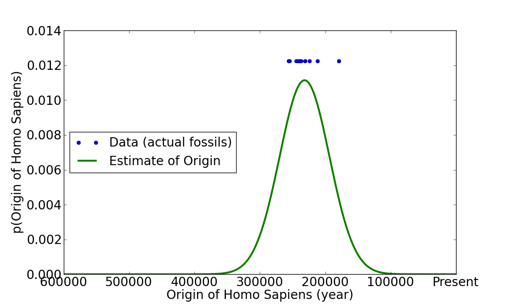
\includegraphics{blah2-2011-01-29-11-35.png}
\caption{Hypothetical distribution of ages for *homo sapiens*.}
\end{figure}

The details of this are unimportant, because the picture is pretty clear
regardless of the details. A few observations are in order here:

\begin{enumerate}
\def\labelenumi{\arabic{enumi}.}
\itemsep1pt\parskip0pt\parsep0pt
\item
  Our "best guess" is around the middle of this distribution, but it
  really can't be interpreted as "homo sapiens originated 250,000 years
  ago" as it might read in a newspaper
\item
  there are many possible values for the origin time of *homo sapiens* that lie well outside of our data yet have non-zero probability.  This means that these values could very well be the truth, and we are being up front about it.
\end{enumerate}

Now, we have a new paper that adds another fossil much older than than
the previous ones, around 340000 years ago. Currently, newspapers often
make claims like ``origin of homo sapiens 150\% older than originally
thought'', or ``estimates of the origin of humans overthrown by new
data''. How might it look with the uncertainties plotted?

\begin{figure}[htbp]
\centering
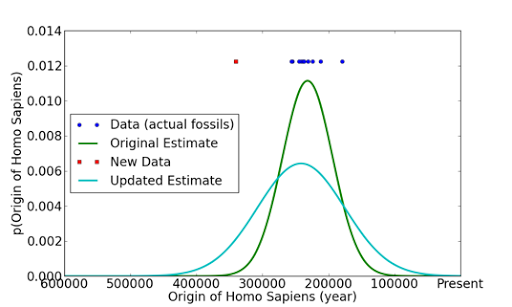
\includegraphics{blah3-2011-01-29-11-35.png}
\caption{Hypothetical distribution of ages for *homo sapiens*, with one added data point.}
\end{figure}

There are a number of lessons that can be read from this.

\begin{enumerate}
\def\labelenumi{\arabic{enumi}.}
\itemsep1pt\parskip0pt\parsep0pt
\item
  the new data updates our "best estimate" by only a little - the old
  data, combined with the new data, are used for the estimate
\item
  our uncertainties have widened - by having a larger range of data, our
  uncertainties may have increased with new data.
\end{enumerate}

In reality, estimating an origin (first event) will update a bit
differently than this example shows. For example, the uncertainties in
the right-half of the distribution may not be affected at all by an
older observation. If this data were in medicine, however, and we were
estimating the effect of some new treatment, then the update would be
very similar. A single result of a strong effect may not increase our
best estimate for that effect by a huge amount. The uncertainties in
many medical treatments, or dietary recommendations, straddle the
origin: there is significant probability for \emph{no effect}. It would
be fruitful to see the plot of uncertainties, pushed a little this way
and that, updated in perhaps a wiki style by scientists as new data come
in. There would be many lessons, all of which would help the public
understanding of science.

\begin{enumerate}
\def\labelenumi{\arabic{enumi}.}
\itemsep1pt\parskip0pt\parsep0pt
\item
  observations rarely overturn well-supported scientific understanding
\item
  not all topics have equal uncertainties - doubting everything the same
  amount is not rational
\item
  certainty is never an option, but sometimes the uncertainty is so low
  that there is a practical certainty
\item
  nature itself, not authority, determines our best guess and some of
  our uncertainty
\item
  if the thing you are measuring has a small effect, then you should
  expect a series of measurements of the effect to change sign: bran is
  good, bran is bad, bran is good, etc\ldots{}. This doesn't mean that
  the scientists are waffling, it only means that the effect is small
  and difficult to detect - and probably meaningless.
\end{enumerate}

I think the public could learn to, at least qualitatively, understand
and use plots like these. Perhaps there is a better way to display it
that does not do violence to the truth, and we'd be open to that. We
think getting in the habit of making plots like this would be good for
the scientist as well, forcing them to address and communicate the
actual uncertainties in their claims. When we explore specific religions
topic like miracles, this sort of thinking and communication of data
could be critical.

\section{Personal Revelation as
Evidence}\label{personal-revelation-as-evidence}

The definition of personal revelation is the idea that God speaks
directly to an individual, who then communicates their message to
others. Unfortunately, there is never any way to confirm personal
revelation, so can it be used as evidence for God? yes, but not very
good evidence. This is due to the combination of two things:

\begin{enumerate}
\def\labelenumi{\arabic{enumi}.}
\itemsep1pt\parskip0pt\parsep0pt
\item
  The prior probability for God is low (\(P(H)\ll 1\)) and,
\item
  The probability that someone would make the claim of divine attention
  even if there is no divine is substantial
  (\(P(C|\mathbf{not}\,H)\approx 1\))
\end{enumerate}

The second point is because there is both a vested interest for someone
to distort a message or claim divine support. In addition it is also
quite common for people to mistakenly attribute agency to non-agent
driven events as well as to see patterns where there are none. These
common human traits give rise to the following relationships,

The probability of the God hypothesis (\(H\)) given the claim of
personal revelation (\(C\)) is

\[P(H|C) = \frac{P(C|H)P(H)}{P(C)}\]

The various terms, as discussed above, are

\begin{eqnarray*}
P(C|H) &\approx& 1 \\
P(H) &\ll& 1 \\
P(C) &=& \underbrace{P(C|H)P(H)}_{\rm small} + \underbrace{P(C|\mathbf{not}\, H)P(\mathbf{not}\, H)}_{\rm large}
\end{eqnarray*}

thus

\begin{eqnarray*}
P(H|C) &\approx& \frac{\rm small}{\rm large}\\
&\ll& 1
\end{eqnarray*}

which means that personal revelation is poor evidence for the existence
of God.

\chapter{Faith: A Matter of
Definitions}\label{faith-a-matter-of-definitions}

The word \emph{faith} has many definitions, some which seem conflicting.
However, as it is commonly used, the definitions point to a single
quantity. It is easiest to see this in the exploration of faith from
specific examples.

\section{Introduction to Faith and
Probability}\label{introduction-to-faith-and-probability}

It may be helpful to start with the dictionary definition, and then
follow with a number of statements about \emph{faith} to see where the
common usages fall.

\begin{itemize}
\itemsep1pt\parskip0pt\parsep0pt
\item
  faith (noun)\citep{MerriamWebster2009}

  \begin{itemize}
  \itemsep1pt\parskip0pt\parsep0pt
  \item
    strong belief or trust in someone or something
  \item
    belief in the existence of God
  \item
    strong religious feelings or beliefs
  \item
    a system of religious beliefs
  \end{itemize}
\item
  Now faith is confidence in what we hope for and assurance about what
  we do not see. {[}\^{}Hebrews 11:1, New International Version{]}
\item
  Faith is trusting in, holding to, and acting on what one has good
  reason to believe is true in the face of difficulties. The
  difficulties may be where you have to take an action where the outcome
  is beyond your control. (Tim McGrew){[}Brierley:2014aa{]}
\item
  Belief without evidence. Pretending to know things you do not know.
  (Peter Boghossian)\citep{Brierley:2014aa}
\item
  One of the things that becomes apparent in serious Christian
  literature is that no one uses `faith' in the sense of \emph{believing
  things without reasons}. That might be Richard Dawkins' preferred
  definition - except when he was publicly asked by Oxford's Professor
  John Lennox whether he had `faith' in his lovely wife - but it is
  important to know that in theology `faith' always means \emph{personal
  trust} in the God whose existence one accepts on other grounds. I
  think God is real for philosophical, historical, and experiential
  reasons. Only on the basis of my reasoned conviction can I then
  \emph{trust} God - have faith in him - in the sense meant in
  theology.{[}http://mobile.abc.net.au/news/2014-04-18/dickson-tips-for-atheists/5397892{]}{[}empasis
  in original{]}
\item
  Faith is the excuse people give when they believe something and don't
  have a good reason. When you believe something and have a good reason,
  then you give the reason. And in every other instance, you offer
  something that is faith. - Matt Dillahunty
\end{itemize}

From these few definitions, we can already see a few things. First,
people use the term in different ways, at different times, so it will be
critical that we tack down a particular definition. It is also critical
to recognize which definition someone is using, so we don't
inadvertently straw-man their argument. Second, the two primary
components that seem to make up all definitions of faith are
\emph{belief} and \emph{trust}. Faith seems to not be a synonym of
either, but a particular combination of them with some restrictions -
not all beliefs or acts of trust require faith.

\subsection{Belief, Trust, and Faith}

We have already seen that \emph{belief} is represented mathematically by
\emph{probability}, so where \emph{faith} requires belief we will employ
probabilities. \emph{Trust}\citep{MerriamWebster2009} is ``belief that
someone or something is reliable, good, honest, effective, etc.'' So it
would seem that trust is a subset of belief, like knowledge is a subset,
pertaining specifically to the reliability or goodness of the thing
believed.

Faith, however, seems to go a bit further than trust and involve
\emph{action} or the willingness to act. When asked by Peter Boghossian,
\emph{``why don't we say that we have faith in the existence of
chickens?''}, Tim McGrew replies,
\pquote{We are venturing nothing on the existence of chickens. When I believe
that chickens exist and I act on that belief I am not taking any step
that places outcomes I care about beyond my direct control. [In the
case of religion], people are placing the outcome of their eternal
soul out of their control. They are taking a risk where the outcomes
matter. The decision itself is evidenced but the outcome is
uncertain.}

\subsection{Utility - Probability and Action}

Probability relates to belief, a measure of state of knowledge about a
claim or set of claims. We can use the mathematics of probability to
determine the most likely claim, and use it to inform our actions, but
it isn't enough to truly determine the best course of action. For that,
we need to extend the mathematics to include the notion of
\emph{utility}, an extension commonly referred to as \emph{decision
theory}. Because faith seems to involve action or potential actions, it
to will need to be formulated in this way.

Decision theory uses the idea of expected value to aid in making
decisions, defined as\citep{Wikipedia:2015aa}

\begin{quote}
The idea of expected value is that, when faced with a number of actions, each of which could give rise to more than one possible outcome with different probabilities, the rational procedure is to identify all
possible outcomes, determine their values (positive or negative) and the
probabilities that will result from each course of action, and multiply
the two to give an expected value. The action to be chosen should be the
one that gives rise to the highest total expected value.
\end{quote}

The utility values, costs and benefits, could be written in monetary
terms, but need not. One needs only to have a scale to represent how
good or bad an outcome is. The total expected value, also called the
average utility, is just the sum of the individual costs and benefits
associated with possible outcomes, weighted by their probability - more
likely outcomes are weighted more than less likely ones. An example will
help.

The example here is called the ``farmer's
dilemma''\citep{jordaan2005decisions}, concerns a farmer who can plant
one of three crops (labeled \$A, B, \$ and \(C\)) with the possibility
of three different environments out of the farmer's control,
\emph{perfect weather}, \emph{fair weather}, and \emph{bad weather}.
Each of the three crops fare differently in different weather, and thus
provide different costs and benefits to the farmer depending on the
environment. Crop \(A\), for example, does very well in good weather but
very badly in bad, whereas crop \(C\) doesn't do as well but is more
consistent, with crop \(B\) in between. This can be summarized by the
following table of utilities showing benefits (positive) and costs
(negative) for each possible combination:

\begin{tabular}{@{}llll@{}}
\toprule
 & \multicolumn{3}{c}{\textbf{Utility (benefits and costs)}}   \\ \midrule
 & \textit{perfect weather} & \textit{fair weather} & \textit{bad weather}   \\
\textit{plant crop $A$} & 11 & 1 & -3  \\
\textit{plant crop $B$} & 7 & 5 & 0  \\
\textit{plant crop $C$} & 2 & 2 & 2   \\ \bottomrule
\end{tabular}\vspace{.1in}

Any decision the farmer makes must include the probabilities (his state
of knowledge) of the weather environments. At the extremes, it is easy
to see this. If perfect weather is nearly guaranteed, for example, then
planting crop \(A\) is of course the best option, whereas if bad weather
is guaranteed, then planting crop \(C\) is the best. How does one handle
the decision away from the extremes? This is done by asking, what is the
average utility (benefit or cost) for each action, and then choosing the
action which maximizes this. Imagine that the farmer consults a
meteorologist, and they determine the following probabilities for the
weather environment{[}\^{}It is possible in some cases that the
environmental state also depends on the actions taken. This is easy to
add to this framework, but makes this particular example needlessly
complex.{]}

\begin{eqnarray*}
\P{perfect weather}&=&0.1 \\
\P{fair weather}&=&0.5 \\
\P{bad weather}&=&0.4 \\
\end{eqnarray*}

The average utility{[}\^{}Average, or expected, value of a variable
\(U\) is denoted with angle brackets, \(\langle U \rangle\){]} for each
action is simply the sum of the probabilities of each environment times
the utility for that environment given the action, such as

\begin{eqnarray*}
\langle U_A \rangle &=& \P{perfect weather}\times {\rm U}(\mbox{perfect weather}|\mbox{plant crop $A$}) + \\
&& \P{fair weather}\times {\rm U}(\mbox{fair weather}|\mbox{plant crop $A$}) + \\
&& \P{fair weather}\times {\rm U}(\mbox{bad weather}|\mbox{plant crop $A$}) \\
&=& 0.1 \times 11 + 0.5 \times 1 + 0.4\times (-3) = 0.4
\end{eqnarray*}

Performing the same calculation for all of the actions yields,

\begin{eqnarray*}
\langle U_A \rangle &=& 0.1 \times 11 + 0.5 \times 1 + 0.4\times (-3) = 0.4 \\
\langle U_B \rangle &=& 0.1 \times 7 + 0.5 \times 5 + 0.4\times 0 = 3.2 \\
\langle U_C \rangle &=& 0.1 \times 2 + 0.5 \times 2 + 0.4\times 2 = 2.0
\end{eqnarray*}

and the best action would be planting crop \(B\), because it has the
highest expected utility.

The primary point about this process that is relevant to our discussion
of faith is that the process involves two separate entities - the
probability of various states and the value those states are to us given
our actions. This maps directly to the concepts of \emph{belief} and
\emph{trust}, respectively. One can focus on each one individually, but
it is the combination that is important.

Although there are cases where the average utility is a bad guide, it is
a very useful framework to structure a problem. It should be noted that
\emph{utility} does not need to be restricted to money, but can include
things like comfort and discomfort. For example, someone could be
\emph{risk averse}, which means that they put a utility on some
psychological comfort at the expense of some monetary loss. Thus the
utility value would combine both.

\section{Rollercoasters: Faith in Everyday
Life}\label{rollercoasters-faith-in-everyday-life}

Words have meaning, and if we are going to communicate with each other
we need to make sure to use words as carefully as we can. Otherwise,
misunderstandings abound. It seems very common that a word like
``faith'' is used by different people for different ends, and the
definition shifts even within an argument. Take for example, the video
by Rich Spear\citep{Spear:2013aa}. In it, Spear presents a distinction
drawn between ``faith'' and ``belief'', using an analogy of a
roller-coaster - belief in the ride being safe vs trusting it being safe
enough to ride on. Notice that his focus is on trust, and thus on
\emph{action}.

It is clear that one must \emph{at least} believe the ride is safe as a
prerequisite for trusting it. Since when we say we believe
\emph{strongly} in a proposition \(A\) when \(P(A)>0.95\) (or some
other, somewhat arbitrary, high number), we can map this prerequisite to
something like the following

\begin{eqnarray*}
\P{safe} = 0.99 \\
\P{unsafe} = 0.01
\end{eqnarray*}

Once you believe it is safe, do you trust it to ride? This brings in
decision theory, where we mix probabilities with utility measures. You
could believe it to be safe at the \(\P{safe} = 0.99\) level, but still
not trust it ``with your life'' because of the \emph{cost} associated
with being wrong. A utility table might look like

\begin{tabular}{@{}lll@{}}
\toprule
 & \multicolumn{2}{c}{\textbf{Utility (benefits and costs)}}  \\ \midrule
 & \textit{safe} & \textit{unsafe}\\
\textit{ride} & 10 & -1000   \\
\textit{don't ride} & 0 & 0  \\ \bottomrule
\end{tabular}\vspace{.1in}

Calculating the average utility for each action we get

\begin{eqnarray*}
\langle U_{\mbox{ride}}\rangle &=& 0.99 \times 10 + 0.01\times (-1000) = -0.1 \\
\langle U_{\mbox{don't ride}}\rangle &=& 0.99 \times 0 + 0.01\times 0 = 0 
\end{eqnarray*}

so it is better not to ride.

As a result, \emph{trust} requires both belief and a sufficiently
positive net utility. Placed in these terms it is much more clear how
the argument is set up.

\begin{itemize}
\itemsep1pt\parskip0pt\parsep0pt
\item
  when the Spear says that "faith" is like "trust", he is
  already approaching the problem with strong belief, and is assessing
  utility - and he rightly claims that belief is not enough.
\item
  when the atheists say that "faith" is "belief without evidence",
  they are addressing the strength of the evidence to obtain strong
  belief in the first place - and claiming that the evidence is not sufficient.
\item
  when the Spear and others say that "faith is rational" they are either talking about utility, not belief, or they are claiming that the
  evidence is in fact good enough for strong belief, and then
  consequently high utility.
\end{itemize}

In all cases, it seems as if for the religious, utility and belief are
muddled when using the word ``faith''. For the atheist, ``faith'' is
always first and foremost about belief, because even the usage involving
trust has belief as a prerequisite. Perhaps if we frame the problem in
terms of belief (probability) and utility we can clear up the fog
surrounding discussions of the term \emph{faith}.

\section{Faith and Trust}\label{faith-and-trust}

We see the same structure occurring in an ``\emph{Unbelievable}''
podcast\citep{Brierley:2014aa} between theist Tim McGrew and Peter
Boghossian. Because they were not thinking in terms of the framework
presented here, they talked past each other through most of the episode.
In this discussion, Boghossian insists that faith is ``belief without
evidence'' or ``pretending to know things you do not know'', and Tim
McGrew insists that faith is more like trust. The discussion then
devolved into a back and forth with both sides claiming that ``all the
people I know use my definition'', and was generally unproductive. It is
clear, however, that in the expected utility equation,

\begin{eqnarray*}
\langle U_{\mbox{action $A$}} \rangle &=& \P{outcome 1}\times U(\mbox{outcome 1}|\mbox{action $A$}) + \\
&&\P{outcome 2}\times U(\mbox{outcome 2}|\mbox{action $A$}) + \\
&&\vdots
\end{eqnarray*}

Boghossian is focusing on the probabilities (\(\P{outcome 1}\),
\(\P{outcome 2}\), etc\ldots{}) and McGrew is focussing on the utilities
(\$U(\mbox{outcome 1}\textbar{}\mbox{action $A$})\$,
\$U(\mbox{outcome 2}\textbar{}\mbox{action $A$})\$, etc\ldots{})

\subsection{The Discussion}

McGrew says that very few Christians (less than 1\%) would use
Boghossian's definition of faith, ``pretending to know things you do not
know''. We agree that no Christian would \emph{articulate} this
definition of faith, however they may be \emph{functionally} using it,
which we will address later.

McGrew opens with
\pquote{Faith is trusting in, holding to, and acting on what one has
good reason to believe is true in the face of difficulties. The
difficulties may be where you have to take an action where the outcome
is beyond your control.}

The example he gives is jumping out of an airplane, where one has faith
in ones instructor to have packed your parachute properly. Ones act of
jumping draws the distinction between faith and \emph{hope} (if you just
\emph{hoped} your instructor packed it, you wouldn't jump), and the
decision is made in the face of evidence, not despite it or without it.

Boghossian's general strategy is to ask a series of questions, to try to
highlight the critical points. For example, we get the following
exchange: * Boghossian: \emph{``what do people mean when they accuse
someone of having
\texttt{faith\ in\ evolution\textquotesingle{}\ "*?\ *\ McGrew:\ *"You\textquotesingle{}re\ trusting\ in\ something\ that\ you\ cannot\ completely\ verify\ because\ it\ doesn\textquotesingle{}t\ lie\ open\ to\ your\ senses."*\ *\ Boghossian:\ *"what\ do\ people\ mean\ when\ they\ say}I
don't have enough faith to be an atheist'''}? * McGrew: \emph{``They
have belief in something in the face of certain difficulties, where the
weight of the difficulties is greater on one side compared to the
other.''} * Boghossian: \emph{``Why don't we say that we have faith in
the existence of chickens?''} * McGrew: \emph{``We are venturing nothing
on the existence of chickens. When I believe that chickens exist and I
act on that belief I am not taking any step that places outcomes I care
about beyond my direct control. {[}In the case of religion{]}, people
are placing the outcome of their eternal soul out of their control. They
are taking a risk where the outcomes matter. The decision itself is
evidenced but the outcome is uncertain.''} * Boghossian: \emph{``Do you
have faith or evidence that Islam is false?''} * McGrew: \emph{``Why
would I use the word `faith' when I am venturing nothing on Islam? I am
a little bit confused about the framing of the question that way. I
think I have evidence that it is false, but since I am not venturing on
Islam, I'm not sure why the word faith would come in.''}

\subsection{Addressing the Definitions}\label{addressing-the-definitions}

Clearly claims using expected utility require that probability
assignments have already been made, so claims of utility must
necessarily be probability claims as well. When translated into these
more precise terms, both McGrew's and Boghossian's claims begin to make
more sense. It will also show that McGrew is in fact using the
Boghossian's definition, in some cases even while denying it.

\begin{quote}
You have faith that your instructor packed your parachute, as opposed to Peter packing it.  Your act of jumping makes faith more than simply hope (if you just hoped your instructor packed it, you wouldn't jump), and the decision is made in the face of evidence, not despite it or without
it.
\end{quote}

The equations are:

\begin{eqnarray*}
\langle U_{\mbox{jump}}\rangle &=& \P{instructor packed}\times \Ug{instructor packed}{jump} + \\
&& \P{Peter packed}\times \Ug{Peter packed}{jump} \\
\langle U_{\mbox{don't jump}}\rangle &=& \P{instructor packed}\times \Ug{instructor packed}{don't jump} + \\
&& \P{Peter packed}\times \Ug{Peter packed}{don't jump}
\end{eqnarray*}

with a possible utility table

\begin{tabular}{@{}lll@{}}
\toprule
 & \multicolumn{2}{c}{\textbf{Utility (benefits and costs)}}  \\ \midrule
 & \multicolumn{2}{c}{*Who packed the parachute?*}  \\ 
  & \textit{Instructor } & \textit{Peter}\\
\textit{jump} & 100 & -10000   \\
\textit{don't jump} & 0 & 0  \\ \bottomrule
\end{tabular}\vspace{.1in}

For this analysis to work, we would have at least, *
\(\P{instructor packed} \sim 1\): one is nearly certain the instructor
packed the parachute * \(\P{Peter packed} \sim 0\): one is nearly
certain that Peter \emph{didn't} pack the parachute *
\(\Ug{instructor packed}{jump}\gg 1\): good benefit from jumping, with
instructor packing the parachute * \(\Ug{Peter packed}{jump}\ll 0\):
large cost from jumping, with Peter packing the parachute *
\(\Ug{Peter packed}{don't jump}=\Ug{instructor packed}{don't jump}\sim 0\):
neutral gain for not jumping in either case

\subsection{Analyzing the Responses}\label{sec:mcgrewresponse}

Notice, for McGrew to have ``faith in his instructor'', two things must
be true: 1. \(\P{instructor packed} \sim 1\): one is nearly certain the
instructor packed the parachute 1.
\(\Ug{instructor packed}{jump}\gg 1\): good benefit from jumping, with
instructor packing the parachute

McGrew wants to focus on point (2), while Boghossian wants to focus on
point (1). Once seen this way, it is very easy to understand the
responses.

For example, why don't we say that we have faith in the existence of
chickens? Because,

\begin{eqnarray*}
\Ug{chickens exist}{action} \sim \Ug{chickens don't exist}{action}\sim 0
\end{eqnarray*}

for all actions - we have nothing at stake, there is no utility, even if
we are confident that chickens exist (i.e.
\(P(\mbox{chickens exist})\sim 1\)).

Does McGrew have have faith or evidence that Islam is false? McGrew
claims he has evidence that Islam is false, \(\Pg{Islam}{data}\ll 1\),
but is not venturing anything on Islam (or more accurately, on his
choice to not follow Islam), \(\Ug{not-Islam}{action}\sim 0\). Again,
Boghossian sees the first part (the probabilities), yet ignores the
second part (the utilities).

Going back to the exchange, we note, however, that sometimes McGrew is
also using Boghossian's definition:

\begin{itemize}
\itemsep1pt\parskip0pt\parsep0pt
\item
  Boghossian: \emph{``what do people mean when they accuse someone of
  having `faith in evolution'''}?
\item
  McGrew: \emph{``You're trusting in something that you cannot
  completely verify because it doesn't lie open to your senses.''}
\end{itemize}

Now I can think of no way to understand this statement from the
perspective of McGrew's definition:
\pquote{When I act on that belief I am taking some step that places outcomes I care about beyond my direct control.}

What outcomes are you placing beyond your control believing in
evolution? What obvious utility are you weighing in this case? As far as
we can see there is none, and so \emph{faith} in this context is in fact
being used here as ``belief without sufficient evidence''.

\subsection{Priors and Faith}\label{priors-and-faith}

We think this brings in another aspect of faith, which we believe
applies to all of the cases explored so far, and that is that faith is
used only in contexts with low \emph{prior} probability. In this
conversation, they spoke of faith in the context of the supernatural,
extreme activities (i.e.~jumping out of planes), events beyond our
immediate senses - all of which coincide with lower \emph{prior}
probability, and need \emph{more} evidence than is typical to overcome
them. They may, or may not, also have high utility. We don't have faith
in the existence of chickens because the existence of chickens has high
\emph{prior} probability.

Because of this, it makes sense that there are those who are not
convinced by the evidence for things others have \emph{faith} in,
because of the necessary quantity and quality to bring a low
\emph{prior} probability up to a significant \emph{posterior}
probability. For those who are convinced by the evidence, it also makes
sense that they would then focus on the \emph{utility} of the claims.
The problem that arises, however, is a problem with the word
\emph{faith}. Since it is referring to two distinct components, the
apologist can easily switch between them without even noticing it
themselves. Again, we put forward the suggestion to discuss things in
terms of decision theory and avoid words with multiple meanings.

\subsection{Without Evidence}

Although a bit shorter and punchier, the term ``belief without
evidence'' is misleading, even if you know you are focussing on the
probability side of the analysis. The more honest phrase would be
``belief without \emph{sufficient} evidence''. When people say there is
no evidence for something (like God, UFOs, astrology, psychic phenomena,
etc\ldots\{\}), they really mean that there is terrible evidence for
something. Even in the case of something so poorly supported as
astrology, there is \emph{some} evidence for its claims - the
probability is not zero. It may be very small, but one could imagine
evidence in principle that would convince you, which means that the
probability is indeed non-zero. The exaggerated, more simple, phrase of
``belief without evidence'' is counterproductive, especially when the
more accurate phrase, ``belief without \emph{sufficient} evidence'', is
nearly as simple.

\section{Does Science Have Faith}\label{does-science-have-faith}

In his talk, ``Life: Creation or Evolution''\citep{Miller:2009aa}, Ken
Miller makes the point that science should inform faith and faith should
inform science. He cites Paul Davies, a physicist who has an interest in
theism, and whose article ``Taking Science on
Faith''\citep{davies2007taking} takes the position that science itself
is a faith-based activity. Ken Miller points out, and one can confirm in
Paul Davies' article, that there are two tenets in science that are
taken on faith:

\begin{enumerate}
\item
  the universe is ultimately knowable and understandable
\item
  knowledge is better than ignorance
\end{enumerate}

These concepts, however, are fundamentally different than faith, or even
axioms. Even here, it is plain that the claims are referring to the
\emph{belief} part of faith, and not the \emph{trust} part of faith. The
entire phrase ``taken on faith'' is a signal to the listener that this
is so.

The first idea, that the universe is knowable, needs to be a bit more
specific: what does it mean to be \emph{knowable}? Prior to 1900, it was
believed that the pieces of a physical model, such as the force of
gravity, or the electric and magnetic fields of Maxwell were ``real'':
there was one-to-one correspondence between the model components and
things in the real world. Thus, it was believed, that knowing the model
you would know nature. After 1900, with the advent of quantum mechanics,
physical models were evaluated based on their predictive value: those
models that predicted well were good models. It was not believed that
there was necessarily a correspondence between the model components and
the real components in nature. Aspects of the model, such as the wave
function in quantum mechanics, were not believed to be real but simply
useful in making predictions. To know the world is to be able to predict
what would happen.

Let's say we replace ``understandable'' with ``predictable'', a
replacement which we think makes practical sense (how else would you
determine that you understand something?), and is directly in line with
modern physical thinking. Doing this, then tenet (1) ceases to be an
axiom, or something we take without sufficient evidence (``on faith''),
but is observable. If the universe is unpredictable, then all attempts
at making prediction will fail. This is not what we observe at all.
Surely there are still things that are unpredictable, such as the
simultaneous value of the position and momentum of the electron, or the
positions of every molecule of air in this room, but even there we can
make specific predictions about average quantities or the values of
other variables of interest. Practically, the universe has demonstrated
itself to be understandable, on the whole. This is not a matter of
faith.

The second tenet (2) I would wager is too vague. What does ``better''
mean? Better for whom, or for what? Psychologically, one might argue
something akin to ``ignorance is bliss'', and there might be something
to that. If we define, however, ``better'' to be higher standard of
living (longer, healthier, more free life) then knowledge can be argued
to have a demonstrable benefit over ignorance. The results of science
has doubled the life expectancy in the past 100 years, and has allowed
us to live more free and healthy lives. As Carl Sagan says, science
delivers the goods. Is there any convincing argument that ignorance is
better, or that we really can't decide which is better?

There is a danger in using the word \emph{faith} in these contexts. It
can communicate to the unaware that there are things that one should
justifiably believe on insufficient evidence - a direct violation of the
laws of probability. It can also imply, for those who take \emph{faith}
to mean \emph{trust}, that the scientists using the term are somehow
admitting an agency in the universe that they don't intend. It serves
only to propagate sloppy thinking in both the fields of science and
religion.

\section{Another Interaction - McGrath and
Dawkins}\label{another-interaction---mcgrath-and-dawkins}

As part of the ``Root of All Evil'' program, Richard Dawkins conducted
many interviews with theists. One in particular, with theologian Alister
McGrath, deals with the notion of faith\citep{Dawkins:aa}. They start
with a discussion about the term \emph{faith}, and McGrath says

\pquote{
We're dealing with a different situation than, for example, evidence
that the moon orbits the earth at a certain distance
}

and

\pquote{
There are many possible ways of explaining *the world*, and we have
to make the very difficult judgement of which is the best of these
*explanations* $\ldots$ evidence takes us thus far, but then when it
comes to deciding between a number of competing explanations, it is
extremely difficult to make an evidence-driven argument.
}

and

\pquote{
I believe faith is rational, in the sense that it tries to make the best
possible sense of things $\ldots$ even though we believe this is the best
possible sense of things, we cannot \emph{prove} this is the
case $\ldots$ there is a point where *faith* goes \emph{beyond} the
evidence
}

By this point, the reader should be able to tell that McGrath is
employing the \{\em belief\} part of the expected utility form of
\{\em faith\}. One wonders in these cases why he doesn't simply talk
about evidence, and the weight of probabilities? Historians, for
example, don't use the word \emph{faith} even though they deal with
probabilities, some of which are highly uncertain. Scientists all the
time deal with probabilities, without invoking the word \emph{faith} in
any paper.

Further, McGrath ignores the fact that there already is a proper and
rational method to address the ``decision between a number of competing
explanations'', that \emph{doesn't} go beyond the evidence, and doesn't
claim more knowledge than is justified. What is this method? It's called
the mathematics of probability! So, McGrath is claiming there is a
problem that faith solves, which is not a problem at all, and he is
using the word faith (at the moment) as synonymous with probability.

Why is he doing this? It seems as if it is because McGrath is holding to
a double standard, and shifts the definitions of concepts around
whenever pressed. He doesn't like the notion of believing strongly
without sufficient evidence (which, as we've seen, is one use of the
word faith), so he defines it (at the moment) to be equivalent to
probabilities.

\subsection{Inference to the Best Explanation}

Then McGrath continues to talk about probabilistic reasoning, and says
that with faith one is doing \emph{inference to the best
explanation}, given a number of competing multiple explanations. As we
stated earlier, if all he means is that faith is probabilistic
reasoning, then we don't have an argument - except that we think he can
make things more clear. We would contend, along with Dawkins, the
\emph{vast} majority of people do not take it to mean this - even the
notion of \{\em faith\} as \{\em trust\} isn't the same as this.

However, we'd like to challenge his basic premise: that in dealing with
multiple competing explanations that one should try to ``infer to the
best explanation'', and \emph{believe strongly in that
explanation}. A simple example introduced in
Section\textasciitilde{}\ref{sec:atheism_agnosticism} on
page\textasciitilde{}\pageref{sec:atheism_agnosticism}, suffices to see
this. In this example, we have two explanations of the number of stars,
one which says that there is an \emph{even} number of stars and another
that says that there is an \emph{odd} number of stars. Pretty much we
know that, at any given instant, one of these \emph{must} be true.
However strong belief in either one is completely unwarranted - there is
simply no way to know. From a probabilistic framework, we express this
as

\begin{eqnarray*}
P({\rm odd}) &=&0.5 \\
P({\rm even})&=&0.5
\end{eqnarray*}

However, it is worse than that. Let's say we had a smidgen of evidence
toward the even-star model, such that we had:

\begin{eqnarray*}
P({\rm odd}) &=&0.499995 \\
P({\rm even})&=&0.500005
\end{eqnarray*}

Even though there is a \emph{best} explanation here (\emph{even} is
slightly more probable than \emph{odd}), and we have the exact
probabilities, it is \emph{still irrational} to hold strong belief in
either explanation. One really does have to look where the weight of the
probabilities lay. Inference to the best explanation fails as a guiding
principle in the face of uncertainty, and is not well defined in all
contexts.

What is happening here is that on the face of it, ``inference to the
best explanation'' sounds like a great thing - something we should
always strive for. However, when you look at what it \{\em actually\}
means, it falls short unless you are in a situation where the best
explanation is also very probable. Strong belief is only justified when
the claim is very probable, not just that is is the most probable
amongst a number of (possibly nearly equivalent) alternatives.

\subsection{Shifting Sands}\label{playing-dodgeball-with-an-apologist}

One of the benefits of seeing these arguments in the light of the
framework of probability is that it makes one sensitive to shifting
definitions. We saw that earlier in
Section\textasciitilde{}\ref{sec:mcgrewresponse} where Tim McGrew
changes his usage of the term \{\em faith\} depending on the response.
Here, McGrath does the same thing.

First it was
\texttt{faith\ is\ reasonable\textquotesingle{}\textquotesingle{},\ based\ on\ evidence,\ going\ beyond\ the\ evidence\ to\ the}inference
to the best explanation'' and that as a result one can have a reasonable
faith in God. Then, when asked about his belief in a creator, and the
evidence for it, despite having difficulty with the implied complexity
of such a creator, he says

\pquote{
I want to go back to CS Lewis who says I believe in Christianity as I
believe the Sun has risen, not simply because I see \textbf{it} by
\textbf{by it} I see everything else. Belief in God gives you a way of
seeing the world that makes an awful lot of sense of it.
}

When pressed on what this implies, he says that \pquote{there are many
  reasons I believe in God and that *origins* is not even the
  primary one...religion really isn't much about where things came
  from, about things in the distant past, but really about how things
  are now. How to live your life, how to be moral, etc\ldots{}
  } which then becomes
\pquote{the key reason for believing God is Jesus, that
  there is something *in the Jesus story* that needs explanation.
} and then, this becomes that it is not really about the life of Jesus,
and his historicity, but how he was perceived by his followers - the
significance they saw in the life and teaching of Jesus.

Notice how this keeps shifting? At first, it is about belief, and then
it is about significance (which one could argue is a kind of utility).
Every time he gets pushed on the specific consequences of his statement,
he retreats, redefines, and redirects the conversation.

He doesn't seem to realize that any explanation, even of things
currently, entails assumptions that can be tested - perhaps with
observations about the past. He can't simply say that religion is
\texttt{not\ about\ where\ things\ came\ from\textquotesingle{}\textquotesingle{},\ when\ they\ explicitly\ make\ statements\ of\ origins\ -\ statements\ which\ have\ been\ universally\ discredited.\ The\ atonement,\ for\ example,\ \textbackslash{}emph\{does\}\ depend\ critically\ on\ the\ existence\ of\ Jesus,\ the\ existence\ the}Fall'',
and a creator of the universe - for none of which did McGrath provide
evidence. If Jesus didn't exist as a real person (or even if he was just
an ordinary guy) then it doesn't matter that his followers simply
\emph{believed} that Jesus was God incarnate when determining ones
belief in the doctrine of salvation. The demonstration of the
historicity of the events claimed is \emph{necessary} for the doctrinal
belief. If you don't have strong evidence of the former, then you are
not rational to believe strongly in the latter - you'd be claiming to
know things you could not know.

As a scientist, one takes an idea, and pushes the idea to it furthest
consequences to see where it breaks, or to see what it depends on.
McGrath seems to change the topic whenever this is done - he does not
seem to want to face the very real, specific consequences of his stated
beliefs and refuses to see the connections between the things that may
be confirmable (apparent design in the biology and the universe itself,
historicity of people and events, alleged miracle claims, etc\ldots\{\})
and the things that make him feel good, but are unmeasurable (existence
of heaven, the atonement of sins, etc\ldots\{\}).

\section{I don't have enough faith to be an
atheist}\label{i-dont-have-enough-faith-to-be-an-atheist}

In their book \emph{I don't have enough faith to be an
atheist}\citep{geisler2004don}, Norman Geisler and Frank Turek are
playing with the word \emph{faith} to make a humorous title. In their
book, however, they too exhibit the dual-usage of the word
\textbf{faith} as in \emph{belief} and as in \emph{expected utility}.

\section{Pascal's Wager}\label{pascals-wager}

Blaise Pascal, a French philosopher, put forward an argument referred to
now as
\texttt{Pascal\textquotesingle{}s\ Wager\textquotesingle{}\textquotesingle{}{[}@Wikipedia:2015ac{]}\ for\ the\ religious\ life\ .\ \ The\ argument\ is\ based\ on\ decision\ theory,\ and\ is\ one\ of\ the\ first\ uses\ of\ this\ theory\ on\ any\ topic.\ \ In\ the}Wager'',
Pascal states that people choose to believe or not believe in God, and
the possible environments they find themselves in are the God either
exists or doesn't. He then sets up the utility table,

\begin{tabular}{@{}lll@{}}
\toprule
 & \multicolumn{2}{c}{\textbf{Utility (benefits and costs)}}  \\ \midrule
 & \textit{God Exists} & \textit{God Does Not Exist}\\
\textit{Believe in God} & $+\infty$ (infinite gain) & -1 (finite loss)   \\
\textit{Don't Believe in God} & $-\infty$ (infinite loss) & +1 (finite gain) \\ \bottomrule
\end{tabular}\vspace{.1in}

It is clear then that the best course of action, given this utility
table, is to believe. There are many problems with this argument, some
which impact the mathematics and others that are theological. An example
of the former is the analysis assumes only one possible God - what if
you choose the wrong God? Extending the table to include this would make
the ``best choice'' not as clear cut. An example of the latter is the
idea that one cannot simple \{\em choose\} to believe, and the act of
pretending to believe would go against the dictates of God.

Pascal's Wager is, however, a useful starting point for a discussion and
highlights some of the issues one faces when applying decision theory
too simplistically.

\section{A More Formal Exploration}\label{a-more-formal-exploration}

In the philosophical literature, there are more formal explorations of
these concepts. These explorations can be helped by casting the ideas
into the probabilistic framework. For example, Daniel Howard-Snyder
considers what he calls ``Propositional
Faith''\citep{howard2013propositional}. He immediately recognizes, as we
do here, that the word \emph{faith} has many usages which he clears away
as being not on topic, and focuses on the use of faith in a sentence
like \emph{``A wife might have faith that her marriage will survive a
crisis''} or \emph{``Frances has faith that her young songs will live
long and fulfilling lives.''} Each of these cases has the sentence
structure of ``\(A\) has \emph{faith that} \(B\)''. In his clearing of
other uses, Howard-Snyder removes the following usages, * Faith as a
noun (e.g. ``earnestly content for \emph{the faith}'') * Faith as a
process (e.g.~the process of coming to believe the Gospel as a result of
the Holy Spirit) * Taking something \emph{on faith} (i.e.~taking on
authority or testimony) * Faith as assent to a proposition with
certainty * Faith as a kind of knowledge

It is interesting to see what Howard-Snyder considers propositional
faith, and some of the considerations around it. We believe he is still
using the term inconsistently, in two ways - one which matches the
structure we've been exploring in this book, and the other as a direct
synonym for \emph{hope}. Consider the following case from his paper.
\pquote{Propositional faith does not require `certainty', without any hesitation or hanging back.  A wife might have faith that her marriage will survive a crisis, while harboring doubts about it.  Indeed, propositional faith is precisely that attitude in virtue of which she might possess the inner stability and impetus that enables her to contribute to the realization of that state of affairs, despite her lack of certainty.}

This case matches decision theory quite nicely. The equations are:

\begin{eqnarray*}
\langle U_{\mbox{action}}\rangle &=& \Pg{successful marriage}{action}\times \Ug{successful marriage}{action} + \\
&& \Pg{failed marriage}{action}\times \Ug{failed marriage}{action} \\
\langle U_{\mbox{inaction}}\rangle &=& \Pg{successful marriage}{inaction}\times \Ug{successful marriage}{inaction} + \\
&& \Pg{failed marriage}{inaction}\times \Ug{failed marriage}{inaction}
\end{eqnarray*}

where the probabilities of the outcomes, as well as the utilities,
clearly change with the the possible actions. For example, we expect
action to have a positive effect on the probability of a successful
marriage,
\(\Pg{successful marriage}{action}>\Pg{successful marriage}{inaction}\).

A possible utility table, which reflects the idea that, if the marriage
is successful without action then there was time and resources saved,
but if the marriage failed without action there is a penalty in the form
of guilt over lost opportunity. Obviously there are many complications
that this table overlooks, and should be seen as a basic approximation.

\vspace{.1in}\begin{tabular}{@{}lll@{}}
\toprule
 & \multicolumn{2}{c}{\textbf{Utility (benefits and costs)}}  \\ \midrule
 & \multicolumn{2}{c}{*How is the marriage?*}  \\ 
  & \textit{successful marriage} & \textit{failed marriage}\\
\textit{action}  & 90 & -100   \\
\textit{inaction} &100 & -110  \\ \bottomrule
\end{tabular}\vspace{.1in}

The high positive utility that the wife puts on her successful marriage,
and high negative utility to its failure, directs her to make actions in
her marriage's favor despite having lower probability of its success.
This is the notion of \emph{faith} worked out.

Another case is
\pquote{But one can have faith that something is thus-and-so without entrusting one's welfare to it in any way, as when I have faith that Emily will survive breast cancer but I do not entrust my well-being to her or her survival}
where as far as we can see, the use of \emph{faith} here is completely
indistinguishable from \emph{hope}. There is no utility explicit in the
statement, and the probability is presumed to be low.

\chapter{Considering Miracles}\label{considering-miracles}

\newcommand{\hrb}[1]{\href{http://web.bryant.edu/~bblais/#1}{#1}}

% maybe unbelievable-project-miracles-and-healing-is-it-evidence-for-the-truth-of-christianity.html}

% maybe \TODO{what do to in the face of serious uncertainty?}  unbelievable-project-john-lennox-debates-science-and-god-has-science-buried-god.html}

\TODO{change the ``I'' to ``we'' here.}

This chapter explores the concept of \{\em miracles\}, and how
probability can be used to describe them and their evidential support.
We defer a discussion of Christianity's foundational miracle, the
Resurrection of Jesus, to Chapter\textasciitilde{}\ref{ch:resurrection}

\section{Introduction to Miracles}\label{introduction-to-miracles}

Perhaps the most influential work on miracles is the chapter
\texttt{Of\ Miracles\textquotesingle{}\textquotesingle{}\ in\ David\ Hume\textquotesingle{}s\ larger\ work\ on\ reason{[}@Hume:1748aa{]}.\ \ It\ is\ also\ one\ of\ the\ most\ often\ \textbackslash{}emph\{misquoted\}\ books\ as\ well.\ \ For\ example,\ Normal\ Geisler\ misquotes\ Hume{[}@Brierley:2008ab{]},\ attributing\ the\ statement}The
evidence for the regular is always greater than that for the rare.'' to
Hume. I think one of the reasons this occurs is that Hume predates
probability theory, so he uses verbose explanations where the modern
reader can insert a single statement. For example, reading Hume's work
on Miracles, it is clear to me that what he intends to say is simply

\pquote{the prior probability for the regular is always greater than the rare}

a bit less pithy, but more correct (although Hume doesn't phrase it
quite like that either). This is at least a factual statement - before
the data, we should believe the regular over the rare. That doesn't
imply that data couldn't convince us of rare events, it only implies
that it is more difficult for data to convince us of rare vs regular
events (i.e.~you need better evidence for the rare).

In an Unbelievable podcast interview with apologist Norman
Geisler\citep{Brierley:2008ab}, Geisler uses the first ``quote'' of Hume
above, and then argues that Hume must be wrong because science already
accepts singular and rare events - the Big Bang, the origin of life, and
macro evolution (this last one is, of course, neither singular nor
rare). Geisler then concludes that miracles can exist! However, seen in
the light of probability theory, it becomes clear.

The prior probability of the events is low:

\begin{eqnarray*}
P(\mbox{Big Bang})\ll 1 \\
P(\mbox{Origin of Life})\ll 1 \\
P(\mbox{Macro Evolution})\ll 1 \\
P(\mbox{Miracles})\ll 1
\end{eqnarray*}

but with data, we have something quite different:

\begin{eqnarray*}
P(\mbox{Big Bang}|{\rm data})\sim 1 \\
P(\mbox{Origin of Life}|{\rm data})\sim 1 \\
P(\mbox{Macro Evolution}|{\rm data})\sim 1 \\
P(\mbox{Miracles}|{\rm data})\sim  0
\end{eqnarray*}

where the data are

\bi
\i Big Bang -
\href{http://www.talkorigins.org/faqs/astronomy/bigbang.html}{a long list}
\i Origin of Life - a
\href{http://en.wikipedia.org/wiki/Abiogenesis}{nice summary} with RNA
world, and autocatalysis \i Macro Evolution - a term not used by
biologists, but
\href{http://www.talkorigins.org/faqs/comdesc/}{another long list} for
evolution \i Miracles - nothing convincing to the scientific community
\ei

So, although all these things \emph{can} occur, only a few of them
\emph{actually} have evidence strong enough to overcome their initial
low prior probability. Hume recognized this for miracles, as was clear
from his writings, although it would have been clearer had he had the
benefit of probabilistic vocabulary.

\section{Critique of Hume}\label{critique-of-hume}

One primary critique of Hume comes from Stanford Encyclopedia of
Philosophy article on miracles\citep{sep-miracles}. As we will see, this
article does very little to modify Hume's conclusions, but we can use it
as a good example of how to use probability mathematics to approach a
philosophical article.

\subsection{Concepts and Definitions}\label{concepts-and-definitions}

The article begins by discussing one of Hume's definitions of a miracle
as
\texttt{a\ violation\ of\ the\ laws\ of\ nature\textquotesingle{}\textquotesingle{}.\ From\ what\ I\ can\ tell,\ their\ main\ critique\ is\ they\ don\textquotesingle{}t\ like\ the\ connotations\ of\ the\ word}law'',
a perspective I share - it is a bit loose terminology, with too many
alternate meanings to be the foundation of a well-defined argument.
Their revised definition is the following:

\begin{quote}
A miracle is an event that exceeds the productive power of nature
\end{quote}

Perhaps this is the scientist in me, and why I am not a philosopher, but
I don't see a striking difference between these two definitions in at
least how they are used. So it seems reasonable to adopt this as a good
working definition.

They go on to clarify a subset of miracle,

\begin{quote}
a religiously significant miracle is a detectable miracle that has a
supernatural cause.
\end{quote}

This clarification is to deal with the following problem, and I'd agree
with at least the sentiment.

\begin{quote}
An insignificant shift in a few grains of sand in the lonesome desert
might, if it exceeded the productive powers of nature, qualify as a
miracle in some thin sense, but it would manifestly lack religious
significance and count not be used as the fulcrum for any interesting
argument.
\end{quote}

I am not sure how, in practice, one would be able to determine a
\texttt{supernatural\ cause\textquotesingle{}\textquotesingle{},\ let\ alone\ establish\ how\ an\ event\ could\ be\ beyond\ the}productive
power of nature'' without committing a fallacy of
\emph{argument from ignorance}, but let's leave that for now.

\subsection{Arguments for Miracle
Claims}\label{arguments-for-miracle-claims}

This section starts with a quick list of the types of evidence and
arguments made for miracles.

\begin{quote}
Many arguments for miracles adduce the testimony of sincere and able
eyewitnesses as the key piece of evidence on which the force of the
argument depends. But other factors are also cited in favor of miracle
claims: the existence of commemorative ceremonies from earliest times,
for example, or the transformation of the eyewitnesses from fearful
cowards into defiant proclaimers of the resurrection, or the conversion
of St.~Paul, or the growth of the early church under extremely adverse
conditions and without any of the normal conditions of success such as
wealth, patronage, or the use of force. These considerations are often
used jointly in a cumulative argument. It is therefore difficult to
isolate a single canonical argument for most miracle claims. The various
arguments must be handled on a case-by-case basis.
\end{quote}

All of these pieces of so-called evidence are the worst kind of
evidence, for which there are countless examples of the same, or similar
evidence use to shore up the claims of other (presumably false) beliefs.
You can think
\texttt{Mormonism\textquotesingle{}\textquotesingle{}\ or}Alien
Abductions'' for nearly every point listed.

They then outline two types of inductive arguments:

\begin{quote}
\begin{enumerate}
\def\labelenumi{\arabic{enumi}.}
\itemsep1pt\parskip0pt\parsep0pt
\item
  the conclusion (in this case that the miracle in question has actually
  occurred) is probable to some specific degree, or at least more
  probable than not
\item
  the conclusion is more probable given the evidence presented than it
  is considered independently of that evidence
\end{enumerate}
\end{quote}

Point (1) is just either specifying either
\(P({\rm miracle}|{\rm data})\) directly or establishing only that
\(P({\rm miracle}|{\rm data})>0.5\). Point (2) is
\(P({\rm miracle}|{\rm data})>P({\rm miracle})\). Point (2) is nearly
useless. For example, you could have

\begin{eqnarray*}
P({\rm miracle})&=&0.00001 \\
P({\rm miracle}|{\rm data})&=&0.001
\end{eqnarray*}

and still have a seriously unlikely hypothesis, even given a factor of
100 increase in probability of a miracle given the data. Thus the
\emph{only} thing that matters must be the actual value of
\(P({\rm miracle}|{\rm data})\).

One such argument for miracles specifies the type of evidence needed to
make one confident that one is talking about a miracle. The article
calls this a ``criteriological'' argument, but all of the arguments
dealt with are probabilistic. What are the criteria, for example? This
one is from Charles Leslie:

\begin{quote}
\begin{enumerate}
\def\labelenumi{\arabic{enumi}.}
\itemsep1pt\parskip0pt\parsep0pt
\item
  That the matters of fact be such, as that men's outward senses, their
  eyes and ears, may be judges of it.
\item
  That it be done publicly in the face of the world.
\item
  That not only public monuments be kept up in memory of it, but some
  outward actions to be performed.
\item
  That such monuments, and such actions or observances, be instituted,
  and do commence from the time that the matter of fact was done.
\end{enumerate}
\end{quote}

One can easily site both the golden plates of Joseph Smith, and also the
events surrounding Roswell, that satisfy all of these. Clearly, there is
an issue with them.

Another common argument is called the ``minimal facts'' approach. The
best summary, and take-down of this argument is on
\href{https://adversusapologetica.wordpress.com/2013/06/29/knocking-out-the-pillars-of-the-minimal-facts-apologetic/}{Matthew
Ferguson's blog}. One essential missing part of the minimal facts
approach is that it only includes \emph{likelihoods} and not
\emph{priors}, and thus fails a basic probabilistic analysis.

\subsubsection{Probabilistic arguments}\label{probabilistic-arguments}

The first form here deals with \emph{testimony}, with the following
assumptions and conventions:

\begin{enumerate}
\def\labelenumi{\arabic{enumi}.}
\itemsep1pt\parskip0pt\parsep0pt
\item
  $T_i\equiv$ the proposition ``Witness $i$ testifies to $M$''
\item
  $P(T_i,T_j) = P(T_i)\times P(T_j)$: independence
\item
  $P(T_i|M)=P(T_j|M)$ for all $i$ and $j$: all testimony is
  equally informative
\end{enumerate}

We then easily derive: \[
\frac{P(M|T_1,T_2,\cdots,T_n)}{P(\sim\!M|T_1,T_2,\cdots,T_n)} = \left(\frac{P(T_1|M)}{P(T_1|\sim\!M)}\right)^n \times \frac{P(M)}{P(\sim\!M)}
\]

The article then spins this in a positive way toward miracles:

\begin{quote}
If independent witnesses can be found, who speak truth more frequently
than falsehood, \emph{it is ALWAYS possible to
assign a number of independent witnesses, the improbability of the
falsehood of whose concurring testimony shall be greater than the
improbability of the alleged miracle.} (Babbage 1837: 202, emphasis
original; cf.\textasciitilde{}Holder 1998 and Earman 2000)
\end{quote}

However, comparing with Hume, it becomes obvious why this spin fails:

\begin{quote}
When anyone tells me, that he saw a dead man restored to life, I
immediately consider with myself, whether it be more probable, that this
person should either deceive or be deceived, or that the fact, which he
relates, should have really happened. I weigh the one miracle against
the other; and according to the superiority, which I discover, I
pronounce my decision, and always reject the greater miracle. If the
falsehood of the testimony would be more miraculous, than the event
which he relates; then, and not till then, can he pretend to command my
belief or opinion. (Hume)
\end{quote}

The first quote implies that the terms \(P(T_1|M)\) and
\(P(T_1|\sim\!M)\) refer to speaking truth vs falsehoods
(i.e.\textasciitilde{}lying), as opposed to speaking correctly vs being
mistaken. In the latter, it is very easy to see why, for certain types
of extraordinary events, we would expect fallible observers to have
\(P(T_1|\sim\!M)>P(T_1|M)\) and further that even \emph{if} witnesses
were in general slightly more reliable than not, we can't expect the
observations to be \emph{independent} in general. In the specific case
of the (anonymous) Gospel writers, there is strong evidence of
\emph{dependence} in the accounts to make this entire calculation
(except in its gross qualitative features) irrelevant.

\subsection{Arguments against miracles}\label{arguments-against-miracles}

Quoting Hume again,

\begin{quote}
The plain consequence is (and it is a general maxim worthy of our
attention), ``That no testimony is sufficient to establish a miracle,
unless the testimony be of such a kind, that its falsehood would be more
miraculous, than the fact, which it endeavors to establish: And even in
that case, there is a mutual destruction of arguments, and the superior
only gives us an assurance suitable to that degree of force, which
remains, after deducting the inferior.''
\end{quote}

This is correct, and is a direct statement of Bayesian reasoning \[
\frac{P(M|E)}{P(\sim\!M|E)} =\frac{P(E|M)}{P(E|\sim\!M)} \times\frac{P(M)}{P(\sim\!M)}
\] where we can use the approximations \(P(E|M)\approx 1\) and
\(P(\sim\!M)\approx 1\) and achieve \[
\frac{P(M|E)}{P(\sim\!M|E)} \approx \frac{P(M)}{P(E|\sim\!M)}
\]

The \href{http://plato.stanford.edu/entries/miracles/}{article on
miracles} continues to try to map this to a philosophical structure
(needlessly, I'd say), with the following ``simple version'' of the
argument:

\begin{quote}
A very simple version of the argument, leaving out the comparison to the
laws of nature and focusing on the alleged infirmities of testimony, can
be laid out deductively (following Whately, in Paley 1859: 33):

\begin{enumerate}
\def\labelenumi{\arabic{enumi})}
\item
  Testimony is a kind of evidence very likely to be false.
\item
  The evidence for the Christian miracles is testimony.
\end{enumerate}

Therefore,

\begin{enumerate}
\def\labelenumi{\arabic{enumi})}
\setcounter{enumi}{2}
\itemsep1pt\parskip0pt\parsep0pt
\item
  The evidence for the Christian miracles is likely to be false.
\end{enumerate}

This is, however, much too crude an argument to carry any weight, since
it turns on a simple ambiguity between all testimony and some testimony.
Whately offers an amusing parody that makes the fallacy obvious: Some
books are mere trash; Hume's Works are *some* books; therefore, etc.
\end{quote}

It's remarkable that such a silly parallel is seriously made. The
structure isn't really parallel at all, so let's make it explicit:

\begin{enumerate}
\def\labelenumi{\arabic{enumi}.}
\itemsep1pt\parskip0pt\parsep0pt
\item
  Books are likely to be trash. (in other words, most books are trash)
\item
  Hume wrote some books
\item
  therefore, Hume's books are likely to be trash.
\end{enumerate}

This is a correct argument, given the premises. If all we knew was that
\texttt{some\ guy\ named\ Hume\textquotesingle{}\textquotesingle{}\ wrote}some
book'', then with all probability (if premise 1. is correct) that book
would be trash. The issue is that, unconsciously, we are inserting extra
information - Hume was a famous philosopher, he had a particular
education, etc\ldots\{\} With this extra information, we would have a
hard time supporting a similar premise as 1. above.

The fact that this is so trivially dispensed with makes one wonder - why
would anyone be convinced by this? Why couldn't the author of the
article see it? It smacks of grasping at straws to try to dispel Hume's
main arguments.

The article continues with some odd re-phrasings of Hume, where the
mathematics is just the single line above. I don't understand all the
work. A strange one is then critiqued with an even stranger statement:
\textgreater\{\}The presumptive case against the resurrection from
universal testimony would be as strong as Hume supposes only if,
\emph{per impossible}, all mankind throughout all ages had been watching
the tomb of Jesus on the morning of the third day and testified that
nothing occurred. Even aside from the problems of time travel, there is
not a \emph{single piece} of direct testimonial evidence to Jesus'
non-resurrection.

Does anyone seriously think that the case against a claim always (or
even usually) takes the form of direct testimony against that claim?
Where is the testimony that Zeus didn't exist? Anyone who can explain
this odd line of reasoning, please chime in.

\subsection{Particular Arguments}\label{particular-arguments}

According to the article, Hume lists a set of conditions needed to make
testimony carry maximum weight:

\begin{quote}
There is not to be found, in all history, any miracle attested by
a sufficient number of men, of such unquestioned good sense, education,
and learning, as to secure us against all delusion in themselves; of
such undoubted integrity, as to place them beyond all suspicion of any
design to deceive others; of such credit and reputation in the eyes of
mankind, as to have a great deal to lose in case of their being detected
in any falsehood; and at the same time attesting facts, performed in
such a public manner, and in so celebrated a part of the world, as to
render the detection unavoidable: All which circumstances are requisite
to give us a full assurance in the testimony of men. (Hume 1748/2000:
88)
\end{quote}

Essentially, he is saying that the methods of science have never
confirmed a miracle. The methods of science help
\texttt{secure\ us\ against\ all\ delusion\ in\ themselves\textquotesingle{}\textquotesingle{},\ remove}suspicion
of any design to deceive others'`, with processes
\texttt{performed\ in\ a\ public\ manner\textquotesingle{}\textquotesingle{}\ that}render
the detection unavoidable''.

It is criticized by noting that some of these conditions can cut the
other way, such as the condition of ``credit and reputation'',

\begin{quote}
It might have been said with some shew of plausibility, that such
persons by their knowledge and abilities, their reputation and interest,
might have it in their power to countenance and propagate an imposture
among the people, and give it some credit in the world. (Leland 1755:
90--91; cf.~Beckett 1883: 29--37)
\end{quote}

This is, essentially, pointing out fallacy of authority - a good
critique. Science, by its processes, attempts to avoid that as well. Of
course, Hume predates modern science, so I think we can forgive him some
sloppiness or poor choice of terminology.

Hume continues to suggest that the religious context of the miracle
claime makes the telling of the miracle story even more likely. This
would increase the probability of obtaining the testimony even if no
miracle happened - \(P(E|\sim\!M)\) increases - making the probability
of a miracle go down. The criticism here? The effect could happen in the
other direction:

\begin{quote}
But as George Campbell points out (1762/1839: 48--49), this
consideration cuts both ways; the religious nature of the claim may also
operate to make it less readily received:

\begin{quote}
The prejudice resulting from the religious affection, may just as
readily obstruct as promote our faith in a religious miracle. What
things in nature are more contrary, than one religion is to another
religion? They are just as contrary as light and darkness, truth and
error. The affections with which they are contemplated by the same
person, are just as opposite as desire and aversion, love and hatred.
The same religious zeal which gives the mind of a Christian a propensity
to the belief of a miracle in support of Christianity, will inspire him
with an aversion from the belief of a miracle in support of
Mahometanism. The same principle which will make him acquiesce in
evidence less than sufficient in one case, will make him require
evidence more than sufficient in the other\ldots{}.
\end{quote}
\end{quote}

I disagree quite strongly with this line of thinking. One of the big
problems with pseudoscience is that it promotes poor thinking in other
domains. Someone who believes in miracles will not find it hard to
believe that the miracle claims of other religions are at least
possible. If you believe in unseen agents, then to move from
Christianity to New Age to Scientology isn't that large of a stretch.
Often, when ones religion is undermined, the typical response is to
switch to another religion! Thus, they are not as opposite as ``light
and darkness''. Poor thinking is poor thinking, regardless of the
context.

\subsubsection{Argument from Parity}\label{argument-from-parity}

Hume brings up miracles in other religions. In a fit of special
pleading, the \href{http://plato.stanford.edu/entries/miracles/}{article
on miracles} retorts,

\begin{quote}
All attempts to draw an evidential parallel between the miracles of the
New Testament and the miracle stories of later ecclesiastical history
are therefore dubious. There are simply more resources for explaining
how the ecclesiastical stories, which were promoted to an established
and favorably disposed audience, could have arisen and been believed
without there being any truth to the reports.
\end{quote}

The argument is quite simple - if there are known cases of miracle
claims where no miracle actually occurred, that increase
\(P(E|\sim\!M)\), making the probability of a miracle go down given
testimony. It doesn't matter whether you have good reasons to believe
there was no miracle for these cases - it undermines testimony of
miracles in general.

\subsection{In conclusion}\label{in-conclusion}

So, as far as I can tell, there is no substantive critique to Hume's
statements about miracles. He lacks the rigor of the mathematics of
probability, but his wording is so straightforwardly translated to it
that I find it difficult to see what the problem is. I also found it
ironic that the entire article, which has been pro-miracle the entire
time, ends with this:

\begin{quote}
For the evidence for a miracle claim, being public and empirical, is
never strictly demonstrative, either as to the fact of the event or as
to the supernatural cause of the event. It remains possible, though the
facts in the case may in principle render it wildly improbable, that the
testifier is either a deceiver or himself deceived; and so long as those
possibilities exist, there will be logical space for other forms of
evidence to bear on the conclusion. Arguments about miracles therefore
take their place as one piece---a fascinating piece---in a larger and
more important puzzle.
\end{quote}

This is pretty much exactly what Hume was saying. Given that there is
always a non-zero probability of the testifier either lying or being
mistaken, one has to establish the evidence for a miracle strong enough
to overcome both the negligibly small prior probability and this
non-zero probability of the testimony being wrong. Since mistakes are a
common human trait, and distortions are also common on testimony,
evidence for miracles according to probability theory, Hume, and all
rational thought have always been found lacking.

\section{How to Approach Miracles}\label{how-to-approach-miracles}

I listened to a
\href{http://donjohnsonministries.org/discussion-with-naturalist-matthew-ferguson-part-1/}{recent
interview}
(\href{http://donjohnsonministries.org/discussion-with-naturalist-matthew-ferguson-part-2/)}{Part
2}) with Matthew Ferguson on the
\href{http://donjohnsonministries.org/}{Don Johnson show}, which I found
pretty impressive. Matthew Ferguson has a
\href{http://adversusapologetica.wordpress.com/}{very interesting blog}
that I just found, and have been enjoying reading.

\subsection{Initial Comments}\label{pandoc-initial-comments}

However, I did find several points in the informal debate that I thought
could be handled better (from my armchair, of course!). Just to note
that although I think that if I were there, I might have been able to
deal with some of the questions better, I also think that nearly all of
the debate was handled much better than I could have done. What struck
me at one point, in
\href{http://donjohnsonministries.org/discussion-with-naturalist-matthew-ferguson-part-2/)}{Part
2}, was Don's zeal for the
\href{http://www.amazon.com/Miracles-Credibility-New-Testament-Accounts/dp/0801039525}{miracles
collection by Craig Keener}
(\href{http://www.uncrediblehallq.net/2012/01/0shou5/review-of-craig-keeners-miracles/)}{review
of Keener's book here}). He seemed to think that because there were
hundreds of thousands of miracle reports, that that was evidence for
their truth. He was, however, quick to dismiss any comparison with other
pseudosciences. Ferguson admits on his blog that the ``debate came off
as a little ambushy'' on this point, because he hadn't read this book,
and clearly couldn't respond to all of them, but I think that misses the
point. I think one can address the miracle claims without being entirely
dismissive (and sounding closed minded) but putting them in their proper
context.

\subsection{Evaluating Miracle Claims - Some Lessons from
UFOs}\label{pandoc-evaluating-miracle-claims---some-lessons-from-ufos}

So in Keener's book, there is a \textbf{huge} collection of claims of
miracles. We could find an equally large collection of UFO sightings.
Now, Don and other Christians would be quick to dismiss UFO sightings as
irrelevant, but I would raise the questions:

\begin{quote}
\begin{itemize}
\itemsep1pt\parskip0pt\parsep0pt
\item
  Given a set of claims, how do we determine whether they are true?
\item
  Are any of them true?
\item
  Do the number of claims contribute to their truth value?
\end{itemize}
\end{quote}

I believe that the methods we use to determine the veracity of UFO
claims can be used to investigate any claims, remarkable or not,
including miracle claims. To start, we clearly we can't personally
investigate every single claim, and thus cannot comment on ones we
haven't investigated except to note where it seems similar to ones that
we have. I have a friend who I managed (over several years) to break of
his UFO enthusiasm - he was convinced by all of these television shows
claiming evidence for alien spacecraft observations and visitations. He
invited me over to his house periodically to watch these shows to get my
reaction. This is the process that I would use:

\begin{enumerate}
\def\labelenumi{\arabic{enumi}.}
\itemsep1pt\parskip0pt\parsep0pt
\item
  I would write down each specific claim - what was \emph{actually}
  being claimed, and what details were there? (names of places, time,
  who saw what, etc\ldots{})
\item
  I would note any initial inconsistencies (for example, there was once
  where, in the interview process, the different witnesses actually
  described \emph{different} things! this seemed to go unnoticed by the
  reporter)
\item
  I would go home, and try to find out as much about the \emph{original}
  details of the events. It would take me probably at least an hour for
  each case, and some I couldn't track down. However, many of them I
  could. I would read the claims again, and the skeptical accounts, and
  the responses to the skeptics. I would try to see what the actual data
  was, how it was collected, when it was reported, etc\ldots{}
\end{enumerate}

What I found for \emph{every} case that I personally investigated was
the following:

\begin{enumerate}
\def\labelenumi{\arabic{enumi}.}
\itemsep1pt\parskip0pt\parsep0pt
\item
  Most of the \emph{actual}, original claims were mundane. Lights in the
  sky, marks on the ground, etc\ldots{}. No hard evidence of anything
  remarkable.
\item
  Misinterpretation of a known object, or objects, in the sky or on the
  ground.
\item
  The reporting of the claims grew more and more remarkable. A
  particularly good example was the
  \href{http://en.wikipedia.org/wiki/Rendlesham_Forest_incident}{Rendelsham
  Forest} UFO case where the initial reports were just lights, and the
  later reports involved spacecraft, alien code-books, etc\ldots{}
\item
  There were serious inconsistencies between reports, or anomalous
  non-reports (i.e.~people who \emph{should} have seen something but
  didn't). A good example of this was a
  \href{http://en.wikipedia.org/wiki/2006_O'Hare_International_Airport_UFO_sighting}{Chicago
  airport sighting} where a small group of people, in a localized area
  of the airport, saw something yet the large number of other people in
  the nearby areas of the airport reported nothing.
\end{enumerate}

I repeat - in \emph{every single case} that I personally investigated,
these points were in evidence. Then I look through something like the
\href{http://files.ncas.org/condon/text/contents.htm}{Condon report}
where they go through something like 30 years of data in the height of
the UFO craze and don't come up with even a single item that is not
mundane in its nature. After that, new UFO claims I see with suspicion
even if I don't check them out. If something seems straightforward to
check out, I might do it, but I don't feel it is my job to investigate
every claim. If there had been even a single case which pointed to
something probably remarkable, I'd have a different attitude.

\begin{quote}
Lesson: if the claims made shrink and disappear at critical and
skeptical investigation, the claim is not likely to be true.
\end{quote}

\subsection{Miracles}\label{pandoc-miracles}

The Catholic Church has a division to investigate miracles, and has
determined that some of them are genuine. However, the Catholic Church
often has significant blinders, and definitely takes a long time to
adjust to obvious mistakes (Galileo anyone?).

Take, for example,
\href{http://listverse.com/2008/07/14/top-10-astonishing-miracles/}{this
site on top 10 miracles}. I've personally researched about 3 or 4 of
these, and it is quite clear that those are definitely frauds (\#1, 2,
3, and 5 I've checked). Yet, do we get any retraction from the Catholic
Church? Do we get \emph{any} hint of skepticism? None at all.

Again, I follow the same steps as above. I do not take someone else's
word, necessarily, and I don't discount them out of hand. The miracles
of Fatima are a great example. First, we have
\texttt{visions\textquotesingle{}\textquotesingle{}\ from\ highly\ impressionable\ children,\ one\ of\ whom\ was\ known\ to\ have\ made\ up\ fanciful\ stories\ in\ the\ recent\ past.\ These\ children\ are\ the\ only\ ones\ who}see'`it,
until the last vision where hundreds claimed to see the ``Miracle of the
Sun''. The problem? The initial stories did not agree, and we only get a
semi-consistent story after the various witnesses spoke with each other
and to a priest collecting the reports. Check out
\href{http://www.csicop.org/si/show/real_secrets_of_fatima/}{The Real
Secrets of Fatima} for the details. All of the elements spoken about
above can be seen - initial mundane experiences, misinterpretation of
known objects (i.e.\textasciitilde{}the sun, and clouds), the
exaggeration of stories in later recollection, serious inconsistencies
in reports and notable non-reports.

The same goes for every faith-healer I've read about. A little digging,
and a little skepticism, and the entire enterprise come crashing down.
Many times it doesn't take much digging!

\begin{quote}
If the truth is there, then it shouldn't retreat under investigation.
\end{quote}

This is not a matter of being \emph{too skeptical}. It is a matter of
not being credulous.

\section{Healing Miracles}\label{healing-miracles}

\TODO{fix the formatting here.}

\subsection{Unbelievable? 17 Nov 2007 - Are miracles evidence for God? -
17 November 2007 -- Miracles and healing - is it evidence for the truth
of
Christianity?}\label{unbelievable-17-nov-2007-are-miracles-evidence-for-god-17-november-2007-miracles-and-healing-is-it-evidence-for-the-truth-of-christianity}

As part of the
\href{https://brianblais.wordpress.com/2013/02/27/unbelievable-project-a-non-believers-armchair-perspective-on-six-years-of-christian-debates/}{Unbelievable
Project}, I am taking notes and ``arm-chair'' responding to each of the
\href{http://www.premierradio.org.uk/shows/saturday/unbelievable.aspx}{Unbelievable
podcast} episodes satisfying a set of
\href{https://brianblais.wordpress.com/2013/02/27/unbelievable-project-a-non-believers-armchair-perspective-on-six-years-of-christian-debates/}{simple
rules}.

For a full RSS Feed of the podcasts
\href{http://ondemand.premier.org.uk/unbelievable/AudioFeed.aspx}{see
here}.

\subsubsection{Description of Episode}\label{description-of-episode}

\begin{itemize}
\item
  Full Title: \emph{Unbelievable? 17 Nov 2007 - Are miracles evidence
  for God? - 17 November 2007 -- Miracles and healing - is it evidence
  for the truth of Christianity?}

  \begin{quote}
  Agnostic sceptic Stephen Pilcher believes that Christian claims to
  healing are tricks of the mind.~ Can John Ryeland of the Christian
  Healing Mission persuade him differently?~ Also features personal
  stories from people who claim to have been miraculously healed.
  \end{quote}
\end{itemize}

\href{http://media.premier.org.uk/unbelievable/ba5b6360-edf3-4218-8878-3292237289f5.mp3}{Download
mp3.}

\begin{itemize}
\itemsep1pt\parskip0pt\parsep0pt
\item
  Justin Brierley - Christian Moderator
\item
  John Ryeland - Christian
\item
  Heather Riley - Christian
\item
  Stephen Pilcher - Agnostic
\end{itemize}

\subsubsection{Notes}\label{notes}

Stephen - \emph{``I'm a church-going, Bible-reading agnostic''}

\textbf{Me - That's pretty funny, because it is very close to what I am.
I am a church-going, Bible-reading atheist. Although I have read the
Bible at least once cover-to-cover a few years ago, I have lost patience
with reading it now. There is so much repetitious and tedious material,
both Old and New Testament, that I find it hard to read for long without
thinking I have better things to do with my time.\\}

Stephen - There are a large number of \emph{``miracles''} that aren't
miracles at all, and non-Christians can have healings as well.

Heather - Her story is at 24:40, in case you want to listen to the
original. Here is a quick summary. She pursued a psychology degree,
studied the paranormal. About 3 or 4 months ago, she went to a
chiropodist (aka podiatrist) who told her that one leg was longer than
another (by an inch). She then went, unplanned, to a religious
gathering. During the meeting the preacher gave her some very specific
information about he from several years ago, some comforting words, and
a moving message. And then he healed the asymmetric leg. She said she
felt like she was \emph{``on show''} and that \emph{``God's really got
to do something''}. She also said that she didn't feel any different,
but a friend of hers observing saw the leg lengthening. So then she went
back to the chiropodist. She determined he was Christian, told the
entire story, he repeated the measurement and then did some more
\emph{robust} measurements, and found no difference in leg length. And
since then, her shoes are no longer asymmetric.

Stephen - People have done studies of faith healings and always come up
short.

\textbf{Me - When I first heard that story, a year or so ago when I
first listened to this episode, I recall being pretty impressed with the
healing. Since then, after much reading, and hearing this again I am
not. (It is interesting that I recall it being more impressive, and if I
never heard the story again, might have started to spread a more
impressive story if I told it again. This is a nice reminder of how
these stories, working with the limitations of memory, can grow in the
telling and quickly become unfactual).\\}

\textbf{\textbackslash{}Anyway, why am I not impressed? There are a
number of little details that she dropped in that I find curious.
Consider two models (there are probably more!):}

\begin{enumerate}
\def\labelenumi{\arabic{enumi}.}
\itemsep1pt\parskip0pt\parsep0pt
\item
  \textbf{There is a God, and he decides to heal this leg, but not other
  ailments, and not her husbands problems. This is hard to reconcile
  even on the face of it, and later in the show she talks about this
  somewhat.}
\item
  \textbf{There is no God, these things don't happen, and there are
  other mundane explanations}
\end{enumerate}

\textbf{\textbackslash{}Turns out that leg-lengthening is a very common
form of \emph{``healing''} in these sorts of situations (see
\texttt{The\ Faith\ Healers\textquotesingle{}\textquotesingle{}\ by\ James\ Randi),\ because\ it\ looks\ impressive\ and\ is\ a\ straightforward\ trick.\ That\textquotesingle{}s\ why\ it\ is\ important\ to\ have\ magicians\ as\ well\ as\ scientists\ investigate\ such\ claims,\ because\ scientists\ are\ terrible\ at\ detecting\ dishonesty\ and\ trickery.\ The\ fact\ that\ she\ had\ no\ idea\ that\ one\ leg\ was\ longer,\ until\ a\ few\ days\ before,\ that\ she\ did\ not\ feel\ the\ healing,\ and\ only\ went\ on\ the\ word\ of\ the\ friend\ because\ she\ was\ expecting\ something\ to\ happen,\ that\ she\ was\ impressed\ with\ the\ \textbackslash{}emph\{}prophecy''\}
that the preacher said, referring to things he would have no idea about.
James Randi speaks about this at length, and shows how preachers will
use planted people, microphones, and other techniques to appear to know
things they wouldn't already know. Even if they aren't being deceptive,
they may hear in conversations with the friends ahead of time about
Heather's problems, and then work it into the \emph{``prophecy''}. When
she goes back to the chiropodist she finds out he is a Christian, and
\emph{before} he redoes the measurement she tells the story. Now, this
chiropodist has a vested interest in confirming the healing, because it
will confirm his worldview. This is why we have double-blind
measurements, because we \emph{know} people bias the measurement, the
reporting, the memory of it because of their worldview. In fact, she
tells that the chiropodist had to do more robust measurements to confirm
the equal leg length. Perhaps there was an error in the first
measurement. Perhaps the first measurement was overestimated. Perhaps it
wasn't, and \emph{she} reported it rounding up (i.e.\textasciitilde{}he
says a bit more than 1/2 inch, she tells her friends around an inch, and
then remembers it as such, etc\ldots\{\}). Perhaps the equipment for the
first test has a bias, which might have motivated him to make the more
robust measurements. There are many possibilities that do not require
dishonesty, deliberate deception, incompetence, and are completely
mundane.}

\textbf{So which model can explain each of these? It seems clear to me
that there are perfectly good mundane explanations for nearly every
detail of the story, that the story is inconsistent even with a
\emph{``real''} healing, and that model 2 is definitely better. What
about her asymmetric shoes, and the pain that occured and went away
after a while after the \emph{``healing''}? My shoes tend to get
asymmetric over time (not with each other, but each pushed off to the
outside) and when I get new shoes, and they are flat, I have a little
pain walking and running that goes away as I adjust. Notice that these
events happened \emph{3 or 4 months ago}. There is no way that her new
shoes would have become asymmetric in that time \emph{anyway}.\\}

John - \emph{``There is an awful lot of anecdotal evidence, and I don't
want to be skeptical of it simply because it is not documented. What
else\ldots{}.is she not telling the truth? Of course she's telling the
truth!''}

\textbf{Me - All we need is a slightly overzealous preacher, a slightly
sloppy chiropodist, and a small amount of congitive bias. It really is
that simple, and it doesn't require us to disparage the character of
\emph{anyone} in the story.}

John - \emph{``How high should we set the bar to know that this is a
proper healing story?''}

John - \emph{``For some people they want to make it so hard to call it a
miracle that nothing could ever satisfy that. I want to take Heather's
story, listen to it, and ask `How did it change her'? If it is a story,
told with integrety, seems to have a lasting effect, of course it would
be better if it were documented, but we don't have the ability to get
the documentation.''}

**Me - I listen to this talk about documentation, and about how it's
*\texttt{so\ hard*}, some people are \emph{``so skeptical''} and I have
to think \emph{``cry baby, cry baby, cry baby''}. I even hear the little
whining voice in my
head.\textbackslash{}\emph{``People should be more believing of my
miracle claims''}, \emph{``You're being too skeptical''}, etc\ldots\{\}
Of course, when it comes to \emph{other} people's miracle claims, they
are just as skeptical! It's only the ones that support their worldview
that they consider for special treatment. Sorry, that's not good enough.
Even Heather points this out, saying that she feels that people are more
skeptical of religious claims than claims of the paranormal (which she
saw in her studies of the paranormal). She's noting, in others, the same
thing she is doing with her worldview. I've posted specifically about
\href{https://brianblais.wordpress.com/2012/09/25/naturalistic-bias-presupposing-naturalism/}{this
problem here}.**

\textbf{\textbackslash{}In science, say you are trying to publish a
paper, and the editor or reviewer returns it saying that they are not
convinced of your conclusions, you don't go
\emph{``Oh, you're being too hard on me, too
skeptical. Getting the documentation for this effect I am claiming
exists is just too hard.''} That is just ridiculous. You find a way to
document it, with careful measurements, and you convince the skeptics if
it is true, or not if it is false. Truth should convince even the
skeptics, especially if you're claiming a large effect.}

\textbf{\textbackslash{}Take the Higgs boson, as an example of an unseen
entity for which we only can get indirect inference of its existence. It
was proposed \emph{50 years ago}, and although people may have thought
it was likely to be there, they didn't \emph{believe} it was there until
the proper measurements were done. Measurements which took decades to
set up, required hundreds of people as a team, and has cost billions of
dollars, just to get the documentation for the existence of something
which doesn't even seem to violate physical law. Think about that next
time you hear someone claim that getting documentation for healing is
hard, or that the effect seems to disappear whenever you look into it
carefully, and that is the reason there isn't any evidence for it.}

\textbf{If the claimed effects of so-called faith-healings are real,
they should be \emph{trivial} to demonstrate, document, and convince the
skeptics.}

\chapter{On the Resurrection of
Jesus}\label{on-the-resurrection-of-jesus}

\section{Is the resurrection 97\%
likely?}\label{is-the-resurrection-97-likely}

Richard Swinburne has
written\citep{swinburne2004existence}\citep{swinburne2003resurrection}
that a thorough probabilistic approach leads one to the conclusion that
the resurrection is at least 97\% likely. His argument is summarized
here. He defines a number of propositions.

\bi
\i \(t\): theism is true - there is a God (of the traditional kind)
\i \(k\): background knowledge of natural theology \i \(P(t|k)\):
probability there is a God (of the traditional kind) given the
background knowledge of natural theology. He suggests (from Chapter 1) a
\texttt{modest\textquotesingle{}\textquotesingle{}\ value\ of\ \textbackslash{}{[}\ P(t\textbar{}k)\ =\ 1/2\ \textbackslash{}{]}\ \textbackslash{}i\ \$c\$:\ the\ claim\ God\ became\ incarnate\ at\ some\ time\ \textbackslash{}i\ \$P(c\textbar{}t,k)\$:\ probability\ that}God
became incarnate at some time'`given that
\texttt{there\ is\ a\ God\ (of\ the\ traditional\ kind)\textquotesingle{}\textquotesingle{}\ and}the
background knowledge of natural theology'`Again, from (Chapter 2) he
suggests a
\texttt{modest\textquotesingle{}\textquotesingle{}\ value\ of\ \textbackslash{}{[}\ P(c\textbar{}t,k)\ =\ 1/2\textbackslash{}{]}\ \textbackslash{}i\ \$P(c\textbar{}k)\$:\ probability\ that}some
God became incarnate at some time'`given
\texttt{the\ background\ knowledge\ of\ natural\ theology\textquotesingle{}\textquotesingle{}.\ \ Mathematically\ it\ is\ related\ to\ the\ other\ terms\ as\ \textbackslash{}{[}\ P(c\textbar{}k)=\ P(c\textbar{}t,k)\ \textbackslash{}times\ P(t\textbar{}k)\ =\ 1/2\textbackslash{}times\ 1/2\ =\ 1/4\ \textbackslash{}{]}\ \textbackslash{}i\ \$e\$:\ historical\ evidence,\ broken\ up\ into\ \ \ \ \ \textbackslash{}bi\ \ \ \ \ \textbackslash{}i\ \$e\_\{1\}\$:\ evidence\ of\ the\ life\ of\ Jesus\ (Part\ II)\ \ \ \ \ \textbackslash{}i\ \$e\_\{2\}\$:\ evidence\ of\ the\ detailed\ history\ of\ the\ Resurrection\ (Part\ III)\ \ \ \ \ \textbackslash{}i\ \$e\_\{3\}\$:\ evidence\ that\ Jesus\ satisfies\ the\ requirements\ for\ divine\ incarnation\ more\ than\ other\ prophets\ (Chapter\ 3)\ \ \ \ \ \textbackslash{}ei\ \textbackslash{}i\ \$f\$:\ claims\ that\ the\ evidence\ of\ the\ strength\ given\ by\ \$e\$\ (also\ broken\ up\ into\ \$f\_\{1\}\$,\ \$f\_\{2\}\$,\ and\ \$f\_\{3\}\$\ \textbackslash{}i\ \$P(c\textbar{}f,k)\$:\ the\ probability\ of\ the\ incarnate\ God,\ given\ the\ evidence.\ \ This\ is\ the\ term\ that\ Swinburne\ is\ ultimately\ interested\ in.\ \ His\ final\ result\ is\ \textbackslash{}{[}\ P(c\textbar{}f,k)\ =\ \textbackslash{}frac\{100\}\{103\}\ =\ 0.97\ \textbackslash{}{]}\ We\textquotesingle{}ll\ see\ how\ he\ gets\ there\ as\ we\ continue.\ \textbackslash{}i\ \$P(f\textbar{}c,k)\$:\ the\ probability\ that,\ if\ God\ became\ incarnate,\ we\ would\ have\ the\ evidence\ we\ have.\ \ Swinburne\ suggests\ the}fairly
low'' number of \(P(f|c,k) = 1/10\) \ei
Now all we need do is apply the rules of probability from these
estimates, and we obtain Swinburnes answer of 97\% probability that God
became incarnate in Jesus given the evidence,

\begin{eqnarray*}
P(c|f,k) &=& \frac{P(f|c,k) P(c|k)}{P(f|k)}\\
P(c|f,k) &=& \frac{P(f|c,k) P(c|k)}{P(f|c,k) P(c|k) + P(f|\sim(c,k)) P(\sim c|k)}\\
&=& \frac{\frac{1}{10}\times \frac{1}{4}}{\frac{1}{40} + \left(\frac{3}{4}\times\frac{1}{1000}\right)} \\
&=& 0.97
\end{eqnarray*}

In his book on the existence of God, Swinburne provides a series of
pieces of evidence, denoted \(e_{n}\), where \(P(e_{n}|h,k)>P(e_{n}|k)\)
or the evidence is more likely with theism than in just the background.
He does, however, state that added assumptions to \(h\) must be added to
account for some pieces of evidence of evil that are less likely under,
what he calls, ``bare theism''.

\pquote{The fact that the [evidence of] evil required additional hypotheses to be added to the hypothesis of theism to save it from disconfirmation meant that the evil
lowered the probability of theism as such (bare theism) from its probability on the evidence taken into account previously. The fact of divine hiddenness did not, how- ever, count against the existence of God.}

Swinburne's calculation follows Bayes' rule

\begin{eqnarray*}
P(h|e,k) &=& \frac{P(e|h,k)P(h|k)}{P(e|h,k)P(h|k)+P(e|\sim h,k)P(\sim h|k)}
\end{eqnarray*}

\pquote{Let us turn now to $h_{2}$. This is the hypothesis that there is no god or gods, but an initial or everlasting physical state of the universe, different from the present state but such as to bring about the present state. But there is no particular reason why an unextended physical point or any of the other possible starting points of the universe, or an everlasting extended universe, should as such have the power and liability to bring about all the features that I have described.}

\bi
\i e1 be ?there is a physical universe?. \i second argument, from e2
(which will be the conformity of the universe to temporal order)
i.e.~subject to temporal order \i e3, etc.. consciousness, morality \ei

No physical model here, just words.

\pquote{Now I suggest that a universe without connections between uni- versals would be simpler than one with connections; and one with simpler patterns of connection would be simpler than one with such complicated patterns of connection that rational beings would not be able to infer the future behaviour of objects by means of the simplest extrapolation from their past behaviour. Among theories of the universe as a whole (which will thus have equal scope), simplicity is the sole indicator of intrinsic probability. It then follows that, if we give it the weight that I have urged that we should (so that a very simple theory is more probable than a disjunction of many more complex theories), it would be very probable that there would be no connections between universals at all?that the universe would be chaotic....Either way, it is going to be improbable that in a Godless universe there will be simple connections between universals, and so simple laws of nature. }

\pquote{The arguments of the previous pages have sought to show just this; and indeed that the probability of order of the right kind is very much greater if there is a God, and so that the existence of such order adds greatly to the probability that there is a God.}

\pquote{If only a very narrow range of laws and initial conditions allow such evolution, then we may say that the universe is ?fine-tuned? for this evolution.}

\pquote{There remains, however, a consensus among physicists that the values of the constants in the laws of standard theory (as opposed to the variables of initial conditions) must lie within very narrow ranges if life is to evolve anywhere in the universe?ranges that include the actual values of the constants and probably a few other small ranges in which the values of several of the constants are different from their actual ones. }

\pquote{But the considerable a priori weight of simplicity suggests that in a Godless universe it is a priori improbable that any one universe will be tuned so as to yield human bodies. With $e$ as the existence of human bodies, $h$ as theism, and $k$ as the evidence of a universe conforming to natural laws, $P(e|\sim h,k)$ is very low.}

\pquote{The laws of Relativity Theory and Quantum Theory, integrated perhaps into a ?Grand Unified Theory? or ?Theory of Everything? by which everything physical might be explained (fully or partially, even if not complete- ly), give not the slightest reason to suppose that some brain state would cause a green sensation or a sensed smell of coffee.}

\pquote{If, when I tried to move my foot, my hand moved instead, predators would soon overtake me. But this correct explanation of why (given that intentions cause brain events) the brain is connected by nerves to the rest of the body in the way it is does not explain why we have intentions to move our bodies at all and why they cause brain events, which is a quite different problem. I conclude that the existence of the most novel and striking features of animals and above all of humans (their conscious life of feeling, choice, and reason, causing connected to their bodies) seems to lie utterly beyond the range of successful scientific explanation.}

How is this possible?

\pquote{I argued in Chapter 6 that there was a significant probability to which I gave the somewhat artificial value of 1/2 that a God would create humanly free agents?that is, beings who could choose how to make important differences to themselves, each other, and the world.}

\pquote{I have been arguing that, by permitting moral evil and bringing about natural evil, God gives us (and animals) a good that he could not give us in any other morally permissible way.}

\pquote{Hence evil provides a good C-inductive argument against the existence of God. But it does not provide a very strong one, for the reason that providing life after death for many humans (not merely those who need compensation) and becoming incarnate to share their suffering are the kinds of act that a good God might well do anyway?for they are good acts (and perhaps good acts of different kinds from the other acts of God that we have been discussing, and maybe even acts of best kinds), whether or not required in order for God justifiably to allow the amount of evil that occurs. (See p. 231 for the goodness of an act of the former kind, and pp. 288?90 for additional reasons that God might have for becoming incarnate.) So, with e as the occurrence of the moral and natural evils known to us, h as the hypothesis of theism, and k as the evidence considered in previous chapters, $P(h|e , k) < P(h|k)$, but the former is not less than the latter by very much.}

Argument from divine hiddenness

\pquote{But, if the good desire is stronger than the bad one and I have a deep awareness of the presence of God (that is, such that God?s existence is not open to question), then the balance of inclination will be to the good and there will be no free choice between good and bad. We will be in the situation of the child in the nursery who knows that mother is looking in at the door, and for whom, in view of the child?s desire for mother?s approval, the temptation to wrongdoing is simply overborne. We need ?epistemic distance? from God in order to have a free choice between good and evil.}

Miracles

\pquote{But although God has reason for bringing these things about, he also has reason for not bringing them about or not bringing them about too automatically in response to human needs....The major such reason is that it is good that humans should decide for themselves whether to warn or convert others, that humans should have some responsibility for the (immediate or long-term) spiritual destiny of their fellows. }

\pquote{My conclusion to this section is that, in so far as we have historical evidence (normally in the form of testimony) to the occurrence of an event E that is such that, if it occurred, it would probably be a violation of natural laws and that is of a kind that there is some probability that a God would have reason to bring about, that makes it more probable than it would otherwise be that there is a God. For a God would be expected occasionally to bring about such events. Yet, if there is no God, there is no significant probability that such events will occur. Evidence that an event is of this kind is evidence that it is an event ?too odd? for science to explain. Hence, with k as the evidence discussed in previous chapters, and e as evidence of testi- mony of the above kind, and h the hypothesis of theism, $P(h|e , k) > P(h|k)$. It will depend on the strength of the testimony, by how much $P(h|e , k)$ exceeds $P(h|k)$. }

\pquote{God may answer the prayers of members of all religions. And many doctrines of one religion are compatible with doctrines of another religion. Christianity incorp- orates most of Judaism, and is certainly happy to recognize the occurrence of its foundation miracles. But there are cases of conflict, and for those cases Hume?s point is correct. It follows that that religion (if any) which has the best authenticated miracles has the best evidence from this source in its support.
}

\pquote{In discussing religious experience philosophers have sometimes made the claim that an experience is evidence for nothing beyond itself, and that therefore religious experience has no evidential value. That remark reflects a philosophical attitude that those philosophers would not adopt when discussing experiences of any other kind. Quite obviously having the experience of it seeming (epistemically) to you that there is a table there (that is, your seeming to see a table) is good evidence for supposing that there is a table there. Having the experience of its seeming (epistemically) to you that I am here giving a lecture (that is, your seeming to hear me give a lecture) is good evidence for supposing that I am here lecturing. So generally, con- trary to the original philosophical claim, I suggest that it is a prin- ciple of rationality that (in the absence of special considerations), if it seems (epistemically) to a subject that x is present (and has some characteristic), then probably x is present (and has that characteris- tic); what one seems to perceive is probably so. And similarly I suggest that (in the absence of special considerations) apparent memory is to be trusted. If it seems to a subject that in the past he perceived something or did something, then (in the absence of special consid- erations) probably he did. How things seem to be (in contingent respects),9 that is how we seem to perceive them, experience them, or remember them are good grounds for a belief about how things are or were. }

\pquote{From this it would follow that, in the absence of special consid- erations, all religious experiences ought to be taken by their subjects as genuine, and hence as substantial grounds for belief in the exist- ence of their apparent object?God, or Mary, or Ultimate Reality, or Poseidon.}

\subsection{What is wrong here?}

This all looks very impressive, but what is wrong with this calculation?
It is easiest to see this with an alternative calculation.

\subsubsection{The Probability of the Resurrection - Calum Miller \&
Chris Hallquist - Unbelievable? - 06 July 2013 -- Is the resurrection
97\% likely as Swinburne
claims?}\label{theprobabilityoftheresurrection-calummillerchrishallquist-unbelievable-06july2013--istheresurrection97likleyasswinburneclaims}

As part of the
\href{http://brianblais.wordpress.com/2013/02/27/unbelievable-project-a-non-believers-armchair-perspective-on-six-years-of-christian-debates/}{Unbelievable
Project}, I am taking notes and ``arm-chair'' responding to each of the
\href{http://www.premierradio.org.uk/shows/saturday/unbelievable.aspx}{Unbelievable
podcast} episodes satisfying a set of
\href{http://brianblais.wordpress.com/2013/02/27/unbelievable-project-a-non-believers-armchair-perspective-on-six-years-of-christian-debates/}{simple
rules}.

See here for a
\href{http://ondemand.premier.org.uk/unbelievable/AudioFeed.aspx}{full
RSS Feed of the podcasts}.

\paragraph{Description of Episode}\label{descriptionofepisode}

\begin{itemize}
\item
  Full Title: \emph{The Probability of the Resurrection - Calum Miller
  \& Chris Hallquist - Unbelievable? - 06 July 2013 -- Is the
  resurrection 97\% likley as Swinburne claims?}

  \begin{quote}
  Christian philosopher Richard Swinburne has used probability theory to
  show that the likelihood of the resurrection of Christ is 0.97.\\
  Calum Miller is a Christian apologist and student of Swinburne. He
  talks about why he believes that probability theory can be used to
  show that the resurrection is highly likely to be true.\\ Chris
  Hallquist is an atheist blogger who argues that the resurrection is
  not well supported by evidence or probability.\\ For more debates
  visitwww.premier.org.uk/unbelievable\\ Join the conversation
  viaFacebookandTwitter\\ For Calum Miller http://www.dovetheology.com\\
  For Apologetics UK http://apologeticsuk.blogspot.co.uk/\\ For Chris
  Hallquist http://www.patheos.com/blogs/hallq\\ Get the MP3 podcast of
  Unbelievable?http://ondemand.premier.org.uk/unbelievable/AudioFeed.aspxor
  ViaItunes\\ You may also enjoy:\\ Unbelievable? 16th April 2011 -
  Biblical evidence for the Resurrection - Bart Ehrman \& Mike Licona.\\
  Unbelievable? 7 April 2012 - Are the Jesus Scandals evidence for
  Easter? David Instone-Brewer vs Bob Price.
  \end{quote}
\end{itemize}

\href{http://media.premier.org.uk/unbelievable/d8367d64-5f9f-496f-967a-ff4659e83027.mp3}{Download
mp3}.

\begin{itemize}
\itemsep1pt\parskip0pt\parsep0pt
\item
  Justin Brierley - Christian Moderator
\item
  Calum Miller - Christian
\item
  Chris Hallquist - Atheist
\end{itemize}

\paragraph{Notes}\label{notes}

\textbf{Me - I was really looking forward to this episode. What was not
to like? Probability theory, ancient religions, evidence for
Christianity\ldots{}bring it on! Unfortunately, it really wasn't that
impressive.}

Calum - \emph{``There's what's called the confirmation of resurrection,
the explanatory power. And this is basically the idea that there is a
lot of evidence which, if the resurrection happened would be expected
but if the resurrection didn't happen, it would be very improbable. And
if this is true, if there really is that kind of evidence, then it
follows from probability theory that our confidence in the resurrection
should be greatly increased by this evidence. *Concerning the
prior*, more extraordinary or extreme events are more improbable to
begin with, and so you would need more evidence to confirm them. So a
lot of the debate about the resurrection comes down to the prior
probability, whether we think it is actually really improbable and that
no possible evidence could ever make us convinced of it.''}

\textbf{Me - He basically has the distinction between the following as
the basis for all of the ``calculation'':}

\begin{enumerate}
\def\labelenumi{\arabic{enumi}.}
\itemsep1pt\parskip0pt\parsep0pt
\item
  \textbf{evidence that, if it existed, would be very common if the
  resurrection \emph{did} happen}
\item
  \textbf{evidence that, if it existed, would be very rare if the
  resurrection \emph{didn't} happen}
\item
  \textbf{the prior probability for the resurrection}
\end{enumerate}

**where he admits that
*\texttt{the\ debate\ about\ the\ resurrection\ comes\ down\ to\ the\ prior\ probability*}.
Anyone doing probabilistic inference knows that it should never come
down primarily to your choice of priors. The data needs to rise above
the prior, and the prior needs to be an honest -ideally objective-
assessment of the pre-data probability assignments or, often, the
initial state of ignorance. By admitting this, Calum is essentially
saying either that:**

\begin{enumerate}
\def\labelenumi{\arabic{enumi}.}
\itemsep1pt\parskip0pt\parsep0pt
\item
  \textbf{the data are not strong enough to constrain a diffuse prior,
  and thus is unconvincing or\ldots{}}
\item
  \textbf{you have to come into the debate with a \emph{sharp} prior
  which admits to a presupposition of the strength of the claim.}.
\end{enumerate}

\textbf{Neither of these stances is convincing in the slightest.}

\textbf{Further, in response to this set up, he ignores the most
important thing in any Bayesian treatment is the set of models that you
are using to compare. You cannot simply test the truth of a single model
in isolation, nor is it generally informative to compare model A true or
false. Instead one wants to set up a list of models, hypotheses,
theories to explain the data and evaluate those multiple models. Instead
of,}

\$latex\textbackslash{}P(\{\textbackslash\{\}rm
resurrection\}\textbar{}\{\textbackslash\{\}rm
data\})\textbackslash{}\$\textbackslash{}and\textbackslash{}\$latex\textbackslash{}P(\textbackslash\{\}mbox\{not
resurrection\}\textbar{}\{\textbackslash\{\}rm data\})\textbackslash{}\$

\textbf{you'd want}

\$latex\textbackslash{}P(\{\textbackslash\{\}rm
resurrection\}\textbar{}\{\textbackslash\{\}rm data\}),
P(\{\textbackslash\{\}rm hallucination\}\textbar{}\{\textbackslash\{\}rm
data\}), P(\{\textbackslash\{\}rm
legend\}\textbar{}\{\textbackslash\{\}rm data\}),
P(\{\textbackslash\{\}rm literary\}\textbar{}\{\textbackslash\{\}rm
data\}), P(\{\textbackslash\{\}rm hoax\}\textbar{}\{\textbackslash\{\}rm
data\}),\$
etc\ldots\{\}\textbackslash{}\textbf{where of course each of these models
would have many details beyond the simple label I'm putting in here. By
being explicit with what you're comparing to, it is easier to see where
the different prior probabilities come in. Are you really going to
suggest that someone rising from the dead is on par, prior to the data,
with a legendary construction given how many legendary constructions
we've seen and how many dead rising we've \emph{not} seen?}

\textbf{What is clear is that all of these other models must, a priori,
be more probable than rising from the dead \emph{even if a God exists}.
Just because you believe miracles \emph{could} happen does not mean that
you believe every miracle claim is true, and given the number of clearly
false miracle claims, the prior probability for any miracle claim must
be quite low - even if you believe miracles actually occur.}

\textbf{Another point about the data which Calum never deals with is
that it should include things we \emph{don't} see, not just things we
do. If we expect something to occur with a claim, and we don't see it,
that is in fact evidence against the claim.}

Chris - Most Christians might discount the claim that the miracles
around African religions seem to disappear in the US and UK because of
lack of faith. Or perhaps the miracle stories around Mormonism. What
makes the miracles of Jesus different than these ones? Once you accept
the idea that resurrection claims can exist quite commonly in a group of
religiously charged people, it is no longer quite so hard to understand
the resurrection claims in the Bible.

Calum - The reports of an empty tomb are exactly what you'd expect if
the resurrection actually happened, and would be unlikely in the case of
a non-resurrection event.

\textbf{Me - Dealing with this is actually very simple. He is correct
that \emph{if the resurrection occurred}, then the report of an empty
tomb would very likely be given, and I would add that it would also be
very likely to be reported in the earliest accounts we have of the
resurrection. Is this what we see? No! The empty tomb is not mentioned
in Paul, neither are the physical visitations, both of which you'd
expect to see if the Resurrection actually occurred. Even the
visitations are not mentioned in Mark! So, from a probabilistic point of
view, this is the exact opposite of what we'd expect to see if the
resurrection actually occurred. In fact the descriptions of the
resurrection get more elaborate and more physical the later the text
(Paul has visions, Mark has no visitations but the empty tomb, Matthew
and Luke have visitations, John has the doubting Thomas story,
etc\ldots{}). This is exactly what we'd expect for legendary
development, or a story that has been embellished over time.}

\textbf{The other thing, is it really all that unlikely to have an empty
tomb story with no resurrection? Notice, I'm not saying to have an empty
tomb, but to have an empty tomb \emph{story}. There are several
different routes to get that. One is as a literary device. I believe
Richard Carrier supports this, as a reference to Daniel. Another is a
deliberate counter to
\href{http://en.wikipedia.org/wiki/Docetism}{Docetism}, to gain favor
and win an argument.}

Calum - \emph{``It is not necessarily helpful to have just some kind of
religious context, it must be the right kind of one. So, for example, I
can see very good reasons why God would want to vindicate Jesus'
teaching by resurrecting him because I think Jesus taught a lot of very
good things, I thought he was (obviously as a Christian) I think he was
a very sincere, a very good person. And I can think of a lot of good
reasons why God would choose Jesus to be a prophet and to become
incarnate in him. Whereas I don't see comparably good reasons why God
would want to vindicate Mormon teaching. Obviously a lot of that is
because I don't know a lot about Mormonism but there's still the
asymmetry there.''}

Chris - The positive evidence for Mormonism is a lot better than for
Christianity. We have signed documents by the early followers and
founders attesting to the miracles. The best we can say about Paul's
evidence is that he had a vision. We have a lot of negative evidence for
Mormonism, to be sure, but if we knew more about Christianity perhaps
things would be different.

\textbf{Me - I would add that we have this \emph{pro-Christian} filter
for all of our documents, a filter called the Middle Ages, where
documents supporting Christianity had a much better probability of
surviving (i.e.~copied) than ones critical of Christianity. The only
reason we have the Nag Hammadi texts is that the monks refused to burn
them, as ordered by the Christian orthodoxy at the time, and instead
chose to store them in a cave. Think about that campaign of whitewashing
for hundreds of years! Actually, the fact that we have so little actual
documentary support for Christianity coming from the first century,
despite this huge bias, to me argues against Christianity.}

Chris- How do you know Jesus was sincere or not? Seems like the same
could be said for Joseph Smith.

\subsubsection{Afterward - a bit about
priors}\label{afterward-abitaboutpriors}

(this section is all \textbf{Me -}, so I won't put it in bold.)

I don't really think that when Calum is referring to priors that he
really means that in the same way as \emph{before the data}. It seems to
me, and I believe Swinburne's analysis reflects this, that the prior for
\emph{this} calculation is really the posterior for a \emph{previous}
calculation regarding the existence and properties of God. This is
perfectly legitimate Bayesian procedure, but it makes the argument a
different one. Because of this,
\href{http://ndpr.nd.edu/news/23553-the-resurrection-of-god-incarnate/}{Swinburne's
calculation} for the probability of God needs to be addressed before we
can even deal with the priors in this resurrection argument. That will
have to be another post entirely, but at any rate Calum did not do it a
service in this debate, having not really gotten to the meat of it when
he could have.

\section{Resurrection and Regression}\label{resurrection-and-regression}

Dan Barker has written an Easter Challenge\citep{Barker:1992aa} for any
Christian to come up with a seamless account of what happened on the day
of the Resurrection.

\pquote{The conditions of the challenge are simple and reasonable. In each of
the four Gospels, begin at Easter morning and read to the end of the
book: Matthew 28, Mark 16, Luke 24, and John 20-21. Also read Acts
1:3-12 and Paul's tiny version of the story in I Corinthians 15:3-8.
These 165 verses can be read in a few moments. Then, without omitting a
single detail from these separate accounts, write a simple,
chronological narrative of the events between the resurrection and the
ascension: what happened first, second, and so on; who said what, when;
and where these things happened.

Since the gospels do not always give precise times of day, it is
permissible to make educated guesses. The narrative does not have to
pretend to present a perfect picture--it only needs to give at least one
plausible account of all of the facts. Additional explanation of the
narrative may be set apart in parentheses. \emph{The important condition
to the challenge, however, is that not one single biblical detail be
omitted.}}

Andy Bannister has written a response to this
challenge\citep{Bannister:aa}, which we must admit is in fact consistent
with every detail of the story and supposed contradiction. In many ways
it is impressive.

\todo{describe his method here quickly}

However, there is a significant problem with the method he employs,
which can be elucidated with an analogy to a situation which commonly
arises in mathematics, in the process of fitting a line to data.

\subsection{Regression}\label{regression}

In linear regression, we might have, say, a handful of data points:

\vspace{.1in}\begin{tabular}{cc}
\toprule
\textbf{X} & \textbf{Y}\\
0.0 & -12.5\\
1.0 & 17.9\\
2.0 & -3.2\\
3.0 & 11.4\\
4.0 & 10.8\\
5.0 & 28.8\\
6.0 & 31.8\\
7.0 & 28.3\\
8.0 & 23.4\\
9.0 & 21.9\\
10.0 & 32.7\\
\bottomrule
\end{tabular}\vspace{.1in}

Which is plotted as

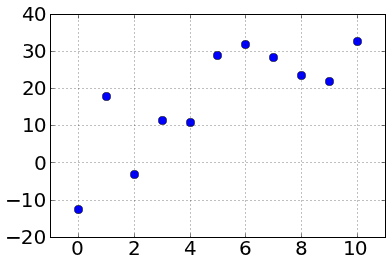
\includegraphics{fig1.png}

When we do a linear regression, we fit to a standard ``\(y=mx+b\)''
form. For this data, the best fit is

\begin{eqnarray*}
y=3.4 x + 0.27,
\end{eqnarray*}

with a mean squared error of 77.9. This difference from the line to the
data is one measure of how well the line compares to the data - lower
values means a better fit, a mean squared error of zero means a
\{\em perfect\} fit.

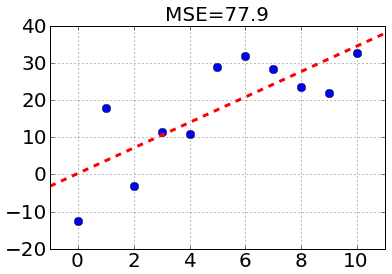
\includegraphics{fig2.png}

Overall, not a bad looking fit. However, if we fit to a more complex
function, say a 10\(^{\rm th}\) polynomial, we can get even better!

\begin{eqnarray*}
y&=&-0.0007039 x^{10}  + 0.0363 x^9 - 0.8051 x^8 + 10.04 x^7 - 77.13 x^6 +\\
&& 376.5 x^5- 1159 x^4 + 2152 x^3 - 2163 x^2 + 891.8 x^1 - 12.54
\end{eqnarray*}

with a Mean Squared Error of \{\em zero\}.

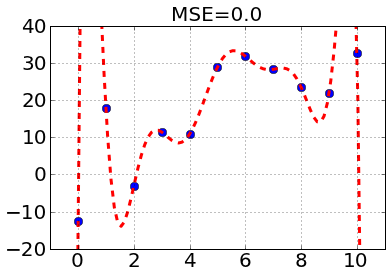
\includegraphics{fig4.png}

In the field of statistics, this is referred to as \{\em over-fitting\},
and is the result of fitting the variation and not the overall pattern.
In other words, it is fitting the meaningless differences from one point
to another by adding a tunable parameter for each detail in the data.
With each new parameter we get a ``better'' fit, by the criterion of
mean squared error, but we lose sight of the meaning. This is the
mathematical equivalent of losing sight of the forest for the trees.

\subsection{Parameters and Ockham's Razor}

When fitting a line, the result is choosing the values of the parameters
that have the highest probability given the data. However, when those
parameters can take on any possible value, the overall probability of
the model is reduced - this is the probabilistic equivalent of Ockham's
Razor which we've seen before in
Section\textasciitilde{}\ref{sec:ockham} on
page\textasciitilde{}\pageref{sec:ockham}.

We make the problem worse by adding more and more parameters, giving
more possible explanatory freedom to our model. The more freedom we have
in choosing the parts of the model, the less explanatory power this
model actually has. One way that statisticians avoid this problem is to
fit the model to half of the data, and see how it works on the other
half - a process called cross-validation. A simple model, like a
straight line, will do about as well on both. An overly complex one will
do well on the data used to fit it, but will do poorly on new data.

\todo{do an example of this in this case}

\subsection{Back to the Resurrection}\label{back-to-the-resurrection}

If we look at Andy Bannister's very clever solution, we notice something
quite interesting: for every single difference between the Gospel
accounts, he adds a detail not found in the story to explain it. One can
pretty much do this for any two accounts that don't say logically
contradictory things, and can be seen as an example of over-fitting.

Another way of looking at it is that, if Bannister had constructed his
story from, say, two of the Gospel stories and then compared it to the
other two he'd have a problem. Even if he took details from all four
accounts, but constructed a story from half of them and then used the
other half to confirm it wouldn't work.

As a result, the Easter Challenge, as phrased, is probably not a very
good one. One can Rube-Goldberg a story together to fit any amount of
details. Perhaps that is the point, to highlight to what lengths someone
has to go to in order to reconcile the four accounts. However, we think
something motivated from cross-validation might be a bit more
persuasive.

\backmatter

\bibliography{main}\bibliographystyle{apalike}

\printindex


\end{document}
